\chapter{Evaluation und Diskussion}

Dieses Kapitel evaluiert, inwiefern das entwickelte Similarity-Hashing-Verfahren für MP4-Container eine zuverlässige Quellenidentifikation ermöglicht, und beantwortet damit Teilfrage~4 der vorliegenden Arbeit (siehe\ Abschnitt~\ref{sec:ff}).\\

TODO: Hier ggf. noch verweis auf relevante Schritte in der Pipeline (7 und 8)


\section{Quantitative Analyse der Erkennungsleistung}

Um die Erkennungsleistung des entwickelten Verfahrens zu quantifizieren, wird für jede forensische Untersuchungskategorie die Fläche unter der Receiver-Operating-Characteristic-Kurve (\(AUC\)) berechnet. Diese Metrik bewertet die Klassifikationsleistung schwellenwertunabhängig, indem sie die True Positive Rate der False Positive Rate über alle möglichen Entscheidungsschwellen gegenüberstellt \cite[S.~2825]{pedregosa_scikit-learn_2011}. Grundlage hierfür ist eine paarweise Ähnlichkeitsberechnung und für jede Untersuchungskategorie repräsentiert ein Source~Digest die n-Gramm-Signatur der Referenzmenge. Jede Testdatei wird anschließend mittels asymmetrischem Tversky-Index verglichen, wobei fehlende Boxen nicht bestraft, zusätzliche Boxen hingegen als Abweichung gewertet werden (siehe \cref{sec:aehnlichkeit}). Der resultierende Ähnlichkeitswert zwischen 0 und~1 dient als Klassifikations-Score, aus dessen Verteilung ROC-Kurve und AUC abgeleitet werden. Um die Vergleichbarkeit zwischen den Kategorien herzustellen, wird zusätzlich der Makro-Durchschnitt aller Einzel-AUC-Werte (\(Mean~AUC\)) ausgewiesen\cite{sklearn_auc_2026}. Dies ist ein in vergleichbaren Container-Forensik-Pipelines etabliertes Vorgehen \cite[Kap.~5]{yang_comprehensive_2025}.


\begin{table}[h]
    \centering
    \begin{tabular}{lll}\toprule
         \textbf{Kategorie der Evaluation}&  \textbf{AUC} (Tversky)& \textbf{Datenbank(en)}\\\midrule
 Gerät& 0.977&VISION\\
         Modell&  0.974& VISION\\
         Hersteller&  0.986& VISION\\
 Aufnahmeart& 0.504&VISION\\
 Social-Media-Platform& 0.971&VISION, EVA-7K\\
 KI-Generator& 0.898&AI\\
 Deepfakes und synthetische Inhalte& 0.546&AI\\ 
 Bearbeitungssoftware& 0.635&EVA-7K\\ 
 KI-generierte Aufnahmen& 1.000&VISION, EVA-7K, AI\\
 Native Aufnahmen& 1.000&VISION, EVA-7K, AI\\ 
 Social Media Aufnahmen& 0.992&VISION, EVA-7K, AI\\
 KI-generierte, native und Social-Media-Aufnahmen& 0.997&VISION, EVA-7K, AI\\ \bottomrule
    \end{tabular}
    \caption{Erkennungsleistung der Container-Auswertung (AUC) über alle Untersuchungsziele}
    \label{tab:auc}
\end{table}


Es wird dargelegt, dass die Klassifikationsleistung des MP4-Similarity-Hashing bei der Quellengeräte- und Markenidentifikation (Gerät: 0.977; Hersteller: 0.986) nahezu identisch zu den Referenzwerten von Klier und Baier ausfällt, welche das MSSH-Verfahren initial für JPEG-Bildstrukturen evaluierten und dort AUC-Werte zwischen 0.949 und 0.992 verzeichneten \cite[Tab. 3]{klier_media_2025}. Dies belegt die erfolgreiche Adaption der n-Gramm-Sequenzierung von statischen Bild- auf hierarchische Video-Container.

Ebenso reihen sich die Erkennungsraten für die Zuordnung zu Social-Media-Plattformen (0.971) nahtlos in die Literatur ein, welche für MP4-Metadaten auf Basis vektorisierter Bag-of-Words- oder Type-Aware-Modelle F1-Scores von rund 0.99 ausweist \cite[Kap. 5]{xiang_forensic_2021}, \cite[Kap. 4]{yang_efficient_2020}.

Die methodische Schwäche des Similarity Hashing offenbart sich hingegen, wie in der Tabelle ersichtlich, isoliert bei der Identifikation der Bearbeitungssoftware. Während das vorliegende Verfahren hier lediglich einen AUC von 0.635 erreicht, erzielen konkurrierende quantitative MP4-Analysemethoden, welche kontinuierliche Werte und exakte Worthäufigkeiten der Container-Boxen in Entscheidungsbäumen verarbeiten, Balanced Accuracies von 0.976 \cite[Kap. 4]{yang_efficient_2020} sowie durchschnittliche F1-Scores von 0.99 \cite[Kap. 5]{xiang_forensic_2021}.

Für die Klassifikation KI-generierter Aufnahmen und die Separation von Deepfakes können in der Literatur keine Referenzwerte herangezogen werden, da die etablierten forensischen Videodatenbanken (VISION, EVA-7K) keine synthetischen Repräsentationen enthalten \cite[Kap. 1]{shullani_vision_2017}, \cite[Kap. 1]{yang_efficient_2020}. Die dargelegten Metriken stellen somit eine neuartige Bemessungsgrundlage in der Container-Forensik dar.

\begin{table}[h]
    \centering
    \begin{tabular}{lrrrr}\toprule
  \textbf{Source Digest}&\multicolumn{3}{c}{\textbf{Anzahl 2-Gramm-Paare}}&\textbf{Größe SD in Bytes}\\
          &   \textbf{Mittelwert}& \textbf{Max}
&\textbf{Min}  &\textbf{Mittelwert}\\\midrule
 \multicolumn{5}{l}{\textbf{Einzelnes Video}}\\
  Alle& 36& 53& 25  &288
\\
          Native Aufnahmen&   39& 53&25&312
\\
          Synthetische Videos&   37& 40&29&296\\
          Social Media&   35& 39&26&280
\\\midrule
 \multicolumn{5}{l}{\textbf{Kategorie}}\\
 Gerät& 40& 54& 25
&320
\\
 Modell& 40& 65& 25
&316
\\
 Hersteller& 39& 69& 25
&312
\\
 Social Media Platform& 42& 54& 36
&333
\\
 AI-Modell& 37& 42& 29
&298
\\ \bottomrule
    \end{tabular}
    \caption{Anzahl der n-Gramm-Paare und Größe des SD (n=2)}
    \label{tab:anzahl}
\end{table}

Anknüpfend an das methodische Vorgehen der Tokenisierung (siehe \cref{kap:feature}) quantifiziert dieser Abschnitt zudem die strukturelle Komplexität der extrahierten Repräsentationen. Durch die 4CC-Bezeichner resultiert für die 2-Gramm-Basis eine fixe Merkmalslänge von acht Bytes. Die statistische Auswertung (siehe \cref{tab:anzahl}) belegt, dass der Similarity Digest einer Einzeldatei aus durchschnittlich 36 einzigartigen Paaren besteht und einen äußerst kompakten Speicherbedarf von im Schnitt 288 Bytes pro Video aufweist. Eine Ausweitung der Token-Sequenz auf größere Intervalle verursacht hingegen eine signifikante Expansion des benötigten Speicherbedarfs. Die Implementierung von 3-Grammen bewirkt einen relativen Anstieg der Digest-Größe um 60 Prozent, während 4-Gramme eine Zunahme um 125 Prozent gegenüber der 2-Gramm-Basis bewirken.

Für die vorliegende metrikbasierte Evaluierung der Klassifikationsleistung (AUC) wird dennoch konsequent das 2-Gramm-Modell angewandt. Es wird dargelegt, dass eine Erhöhung der n-Gramm-Länge auf n=3 oder n=4 keine abweichenden oder feingranulareren Datenstrukturen für die Klassifikation offenbart. Diese Stagnation des Informationsgewinns deckt sich mit den methodischen Beobachtungen von Klier und Baier, welche nachweisen, dass größere n-Gramme zwar das Datenvolumen signifikant steigern, die absolute Anzahl der einzigartigen Similarity Digests pro Untersuchungsziel jedoch konstant bleibt \cite[Tab. 2]{klier_media_2025}. Die 2-Gramm-Sequenzierung bildet folglich das methodische Optimum zwischen algorithmischer Effizienz und forensischer Trennschärfe ab.

%%%

\section{Auswertung nach Kategorien}

Anknüpfend an die quantitative Gesamtbetrachtung erfolgt im vorliegenden Kapitel die detaillierte Evaluation der Klassifikationsleistung, differenziert nach den jeweiligen forensischen Untersuchungskategorien. Zur Gewährleistung einer methodisch belastbaren Auswertung bedarf es einer strikten Partitionierung der zugrundeliegenden Datenbasis in spezifische Referenz- und Testmengen.
Die exakte Konfiguration dieser Evaluierungsszenarien sowie die entsprechende Filterung der Trainings- und Testdaten für die spezifischen Zielsetzungen sind systematisch in \cref{tab:szenarien} zusammengefasst. Diese methodische Abgrenzung soll sicherstellen, dass die in den nachfolgenden Unterkapiteln dargelegten Metriken die funktionale Trennschärfe des Similarity Hashing für die jeweilige isolierte Problemstellung präzise abbilden.

\begin{table}[H]
    \centering\small
    \begin{threeparttable}
        
        \begin{tabular}{>{\raggedright\arraybackslash}p{0.25\linewidth}>{\raggedright\arraybackslash}p{0.34\linewidth}>{\raggedright\arraybackslash}p{0.3\linewidth}}\toprule
              \textbf{Kategorie / Ziel}& \textbf{Testdaten}& \textbf{Trainingsdaten}\\\midrule
              Geräte erkennen\tnote{a}& Unveränderte Originalaufnahmen& Ein Digest für jedes der 34 Geräte\\\midrule
  Modell erkennen\tnote{a}& Unveränderte Originalaufnahmen&Ein Digest für jedes der 28 Modelle\\\midrule
              Hersteller erkennen\tnote{a}& Unveränderte Originalaufnahmen& Ein Digest für jede der 10 Hersteller\\\midrule
  Aufnahmeart erkennen\tnote{a}& Unveränderte Originalaufnahmen&Jeweils ein Digest für Aufnahmetypen Outdoor, Indoor und Flat\\\midrule
            
              Erkennung der Social-Media-Plattform& Native Aufnahmen und Videos, die durch Social-Media-Upload verändert wurden, ohne weitere Bearbeitung& Ein Digest für jede der 5 Social-Media-Plattformen über alle Geräte hinweg\\\midrule
            
              KI-Modell erkennen& Videos, die auf Text- oder Bildvorlagen basieren& Ein Digest für jedes der 11 KI-Modelle\\\midrule
              Erkennung von Image-to-Video und Text-to-Video\tnote{b}& Videos, die auf Text- oder Bildvorlagen basieren& Jeweils ein Digest für synthetische Videos und Deepfakes\\\midrule
            
             	
             Bearbeittungssoftware erkennen& Bearbeitete Videos& Ein Digest für jede der 9 Bearbetungsarten\\\midrule
              Ki-generierte, native und Social Media Aufnahmen erkennen& Alle Videos, die nicht nachträglich bearbeitet wurden& Ein Digest jeweils für alle der 3 Arten: KI-generiert, Social-Media und native Aufnahmen\\\bottomrule
        \end{tabular}

        \begin{tablenotes}\scriptsize
            \item[a] \textit{Lenovo P70A (Device 07)} nutzt nativ kein MP4-Format, sondern speichert das Video als 3GP-Datei und wurde bei der Erkennung von nativen Aufnahmen ausgeschlossen
            \item[b] Reduktion auf die Datensätze der IDs AI01, AI02, AI04, AI07 und AI11, da nur dort jeweils Videos der Kategorie synthetisch und Deepfake zur Verfügung stehen
        \end{tablenotes}

        \caption{Evaluationsszenarien samt Eingrenzung der Trainings- und Testdaten}
        \label{tab:szenarien}
        
    \end{threeparttable}
\end{table}

%%%

\subsection{Native Aufnahmen}

In diesem Abschnitt wird die Quellenerkennung (SCI, Source Camera Identification) für native, unveränderte Videoaufnahmen evaluiert. Das Ziel ist die präzise Differenzierung von Geräten (\cref{fig:auc_geraete}), Modellen (\cref{fig:auc_modell}) und übergeordneten Herstellermarken (\cref{fig:auc_hersteller}) anhand ihrer unverfälschten Container-Struktur. Als Test- und Trainingsdaten dienen hierbei ausschließlich unveränderte Originalaufnahmen aus dem VISION-Datensatz. \footnote{Gemäß Errata (\url{https://lesc.dinfo.unifi.it/VISION/README.txt}) wurden fehlerhafte Aufnahmen der Geräte D03 (Huawei P9) und D19 (Apple iPhone 6 Plus) für die Evaluation nicht weiter berücksichtigt, da eine fehlerhafte Klassifikation als native Inhalte vorlag. Zusätzlich wurde das Gerät D07 (Lenovo P70-A) bei der Erkennung von nativen Aufnahmen ausgeschlossen, da die Containerstruktur im 3GP-Format vorliegenden Dateien nicht zuverlässig extrahiert werden konnte.}

Für die Klassifikation auf Modell-Ebene wird ein aggregierter Source-Digest für jedes der 28 verfügbaren Gerätemodelle generiert. Für die Auswertung auf Marken-Ebene werden die extrahierten n-Gramme sämtlicher Gerätemodelle, die derselben Marke angehören (beispielsweise alle iPhone-Varianten für die Marke Apple), durch eine mathematische Mengenvereinigung zu einem einzigen, umfassenden Marken-Digest aggregiert. Dieses Aggregationsverfahren stellt sicher, dass die signifikante strukturelle Varianz innerhalb einer Produktlinie vollständig erfasst wird. Auf Geräteebene wird für jedes der 34 Geräte anhand ihrer IDs ein Source Digest gebildet.\\

% Gerät

\begin{figure}[!h]
    \centering
    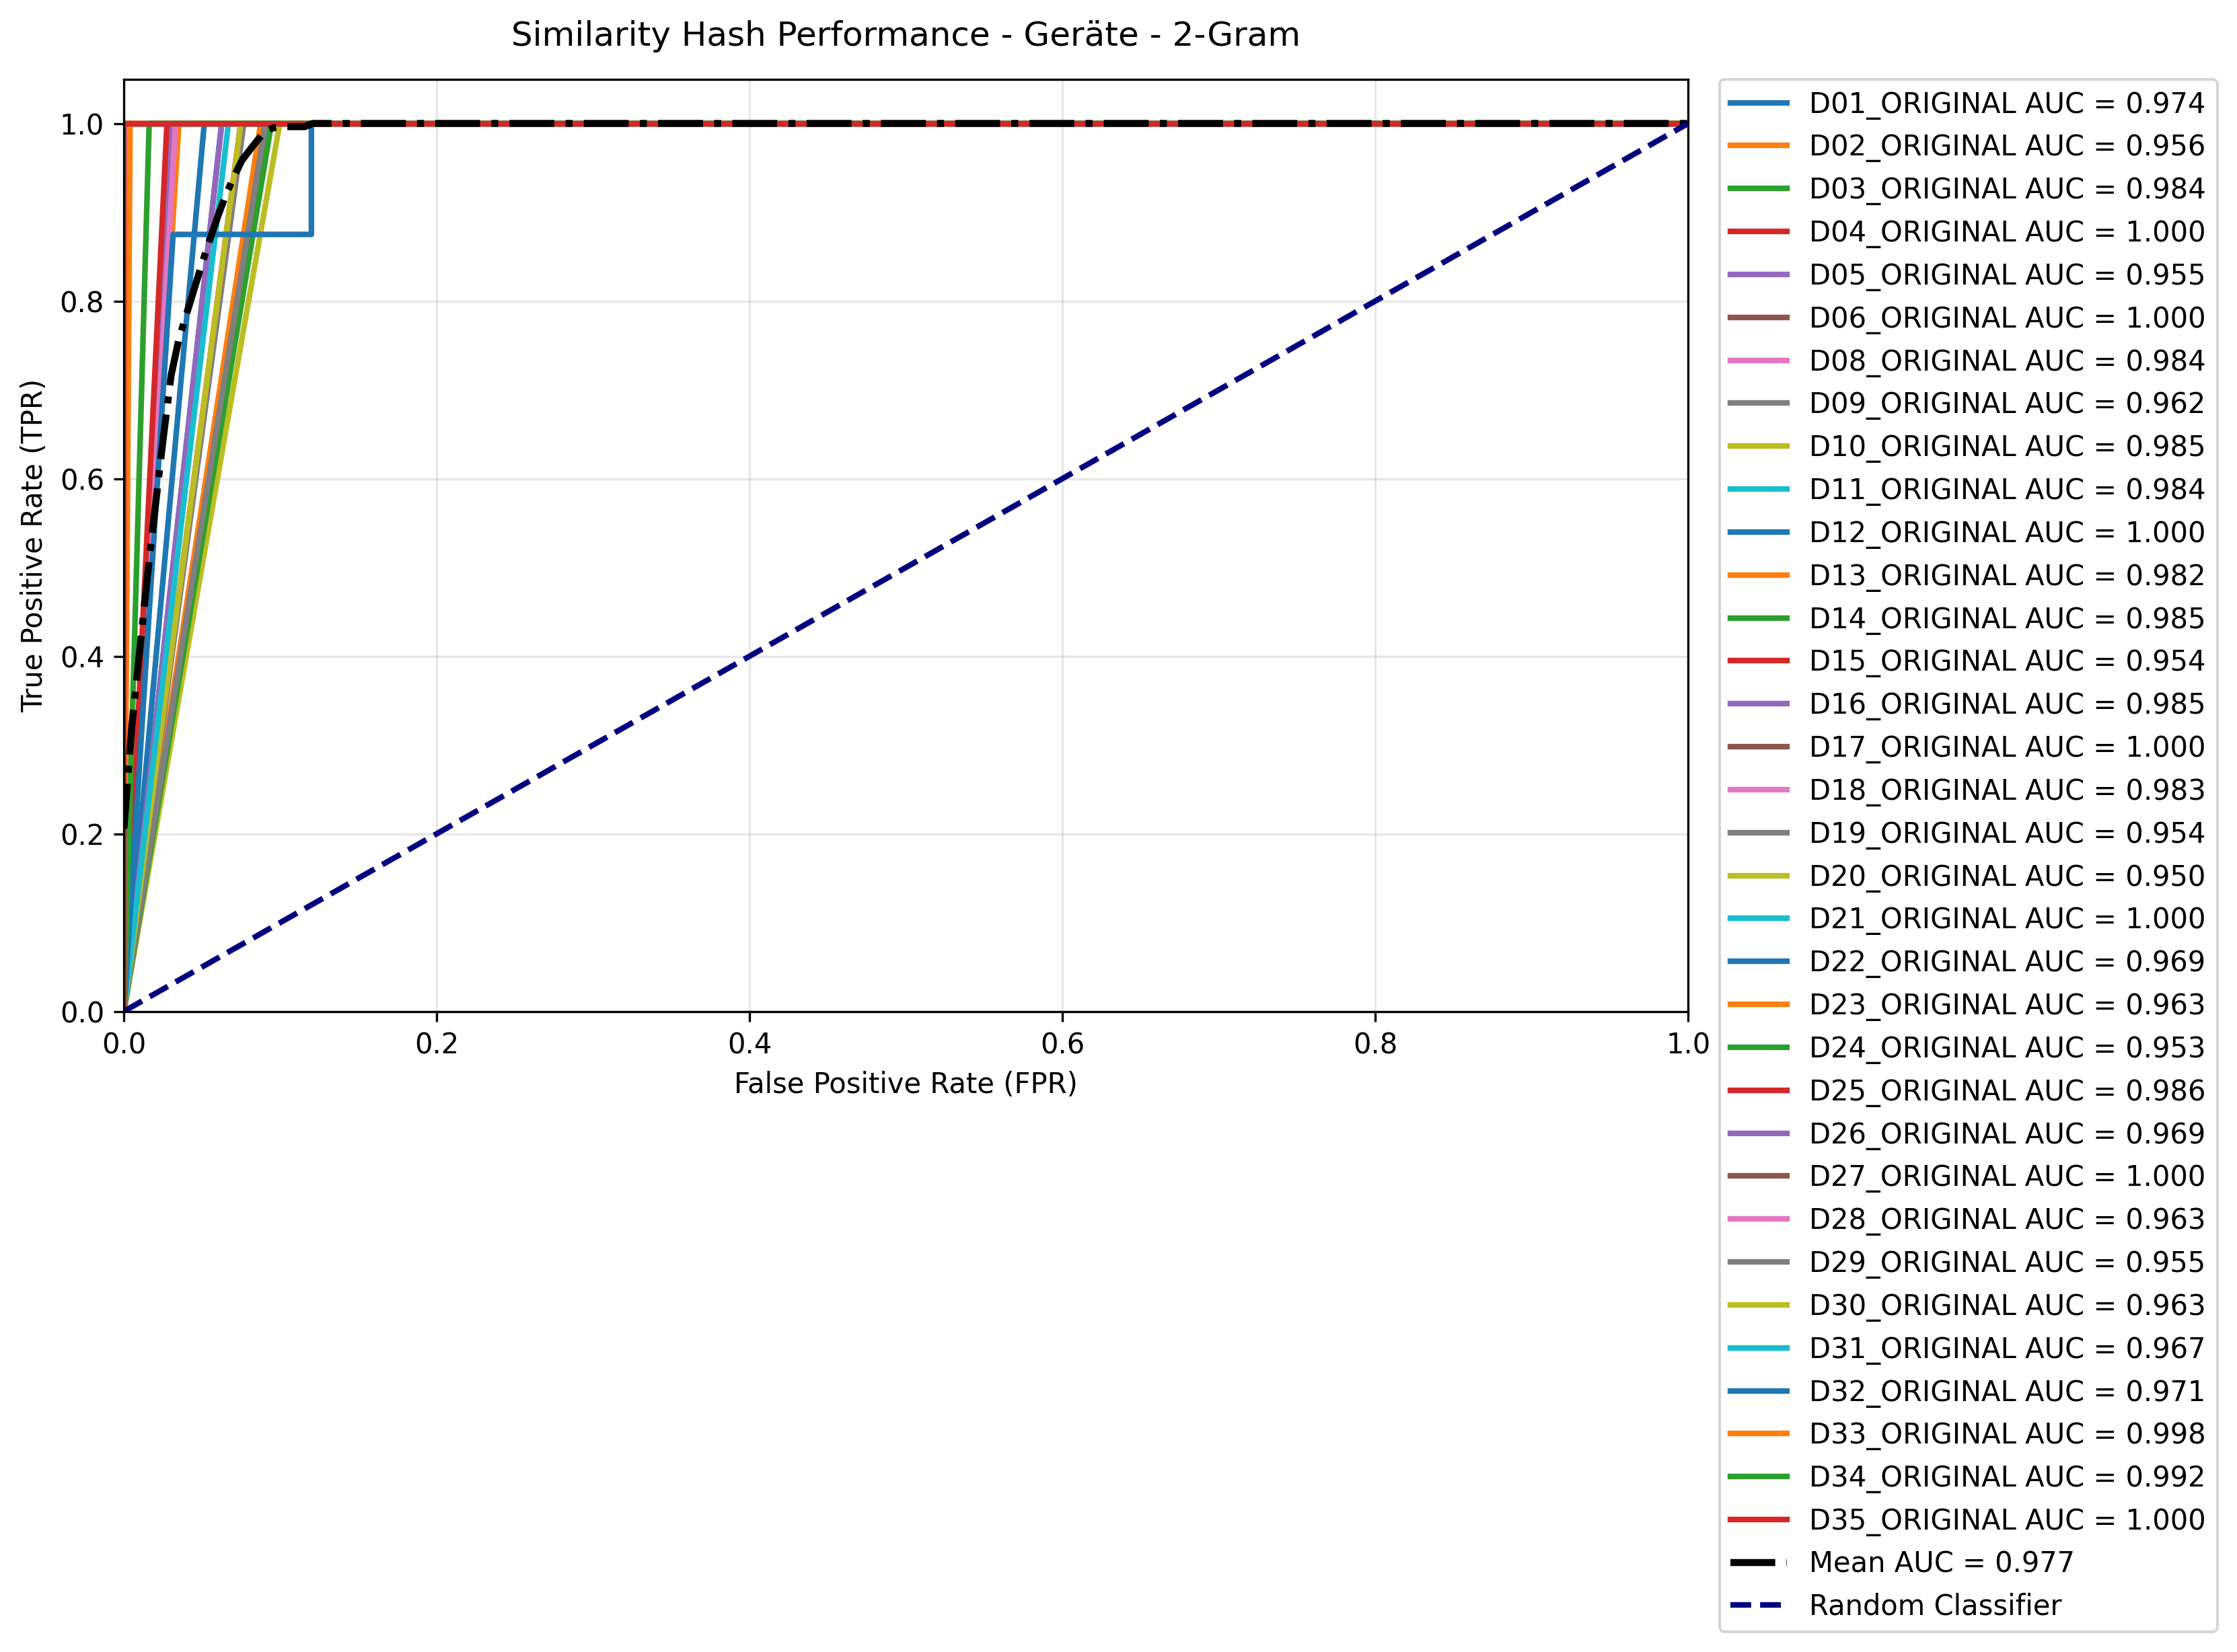
\includegraphics[width=1\linewidth]{grafiken/roc/devices.png}
    \caption{ROC-Analyse und AUC-Werte zur Quellkamera-Identifikation (SCI) auf Geräte-Ebene mittels 2-Gramm-Similarity-Hashing (VISION-Datensatz)}
    \label{fig:auc_geraete}
\end{figure}

\begin{figure}[!h]
    \centering
    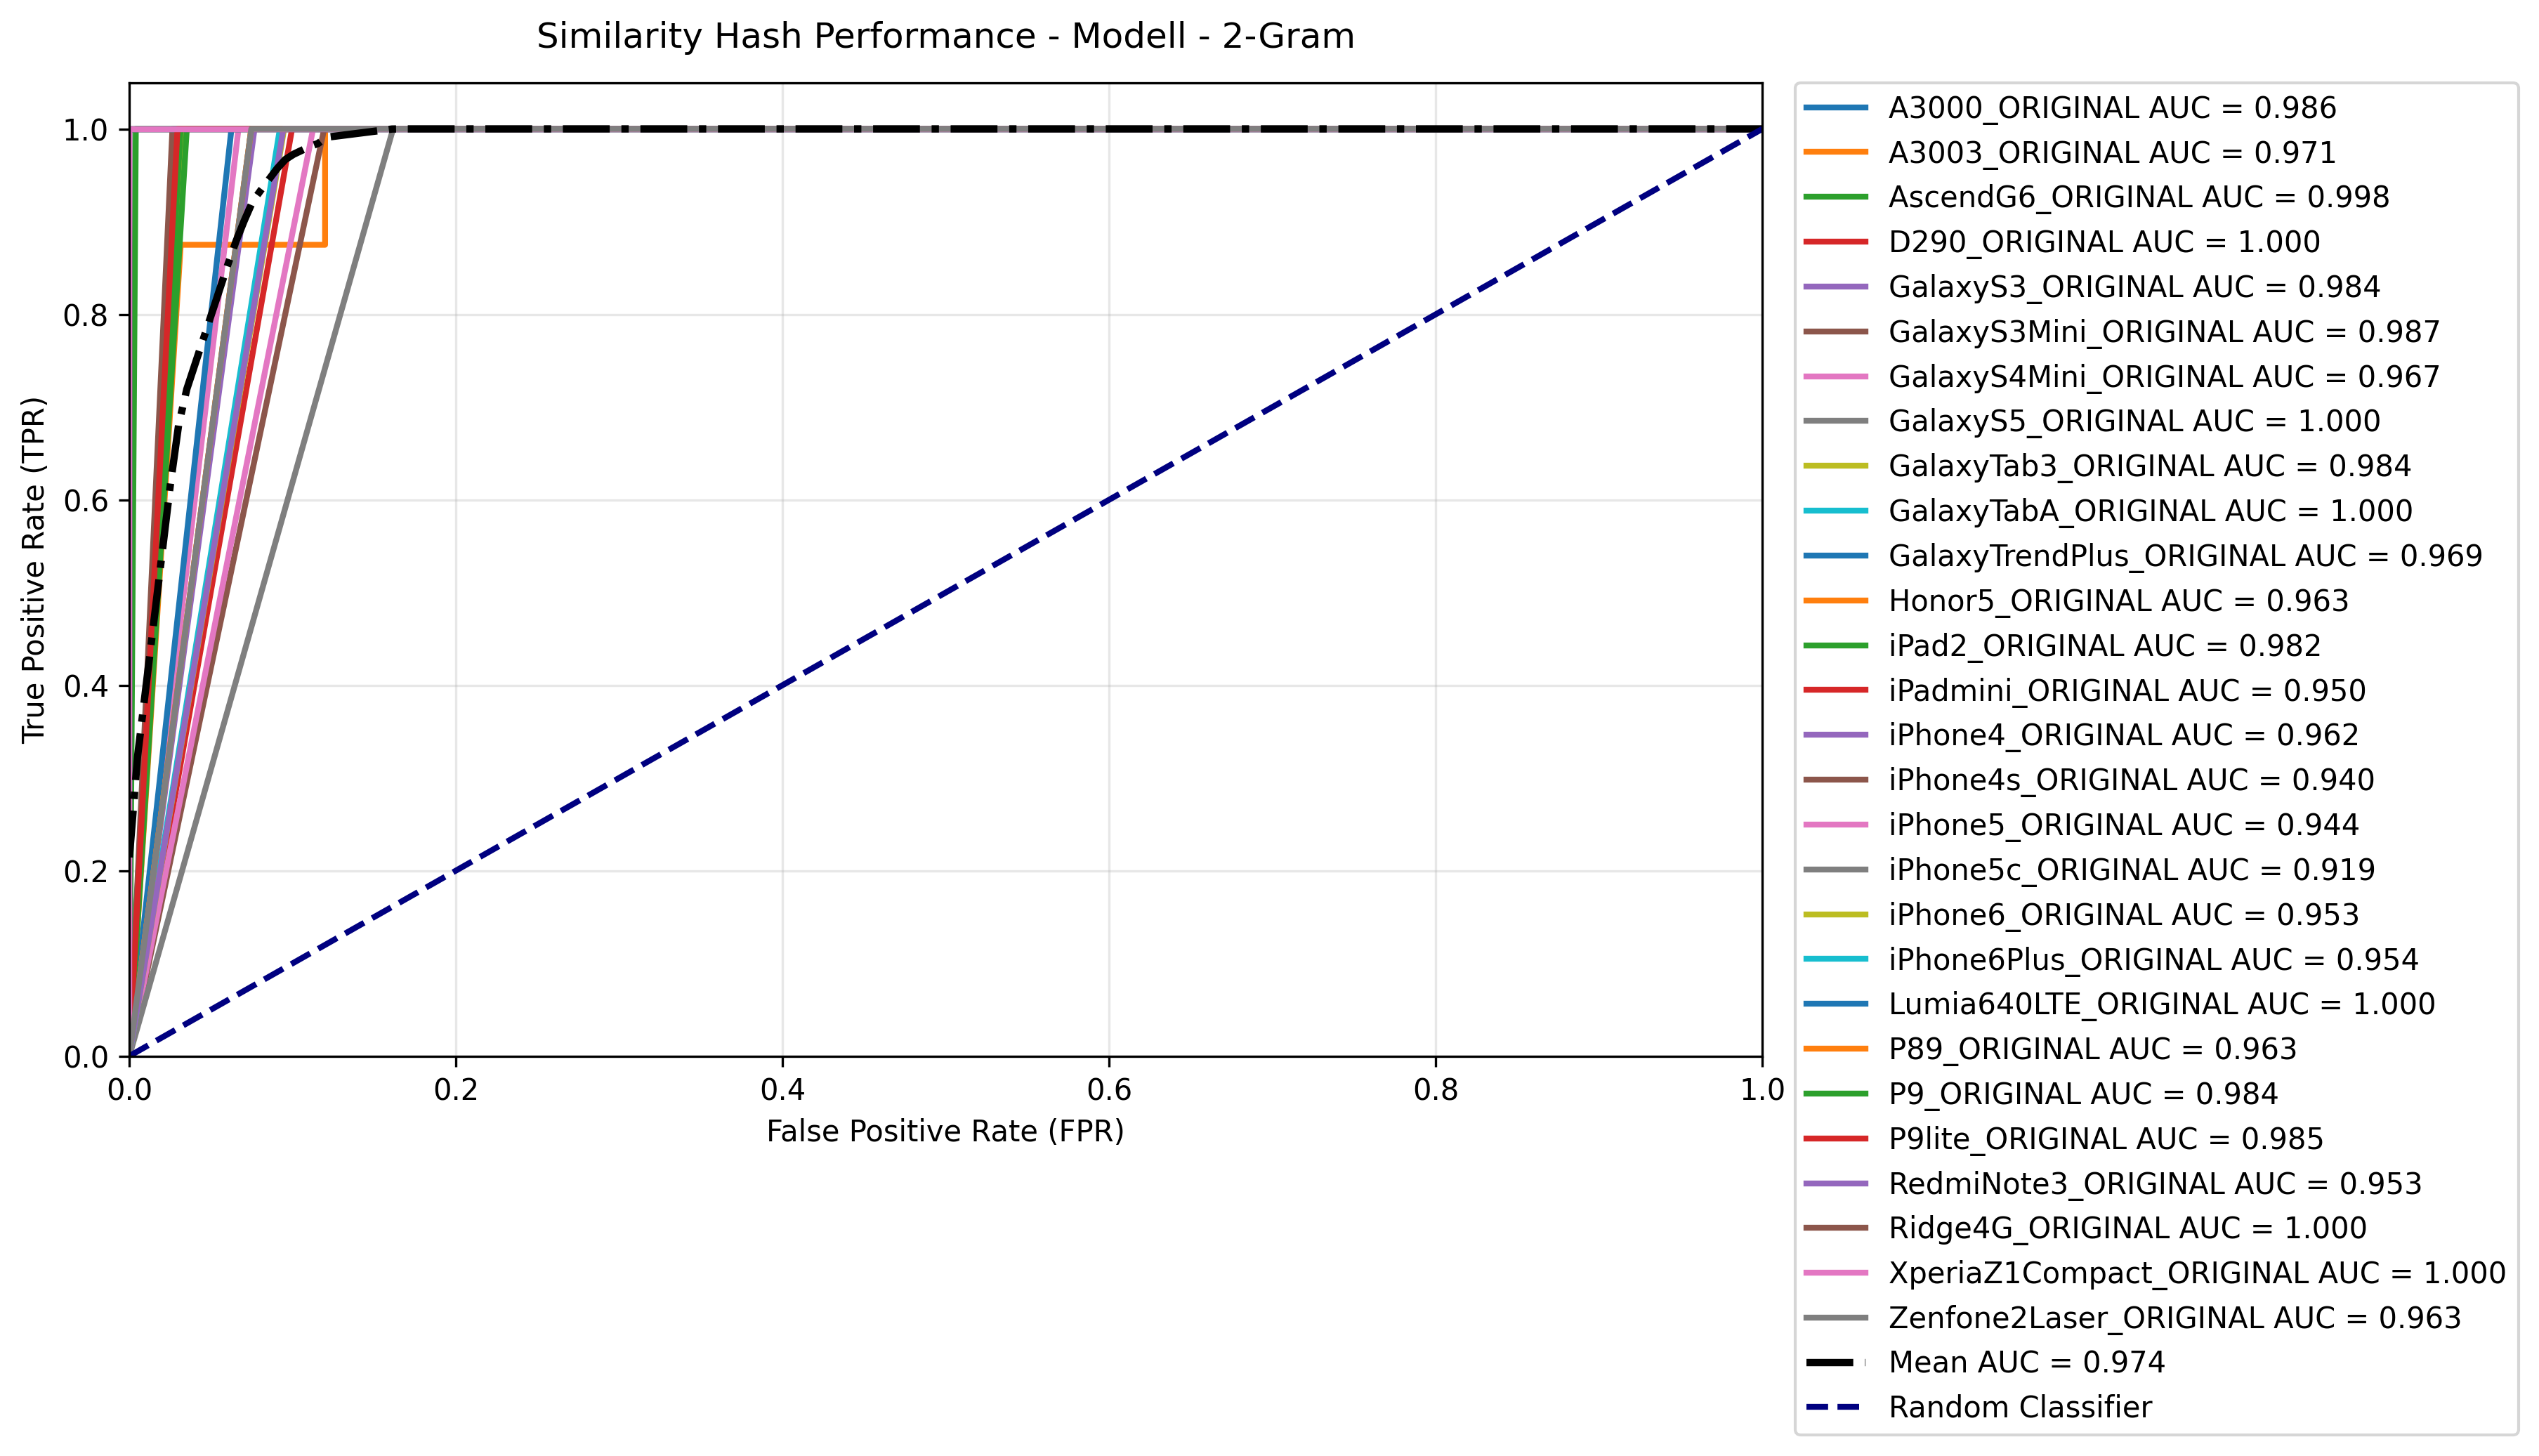
\includegraphics[width=1\linewidth]{grafiken/roc/models.png}
    \caption{ ROC-Analyse und AUC-Werte zur Quellkamera-Identifikation (SCI) auf Modell-Ebene mittels 2-Gramm-Similarity-Hashing (VISION-Datensatz)}
    \label{fig:auc_modell}
\end{figure}

\begin{figure}[!h]
    \centering
    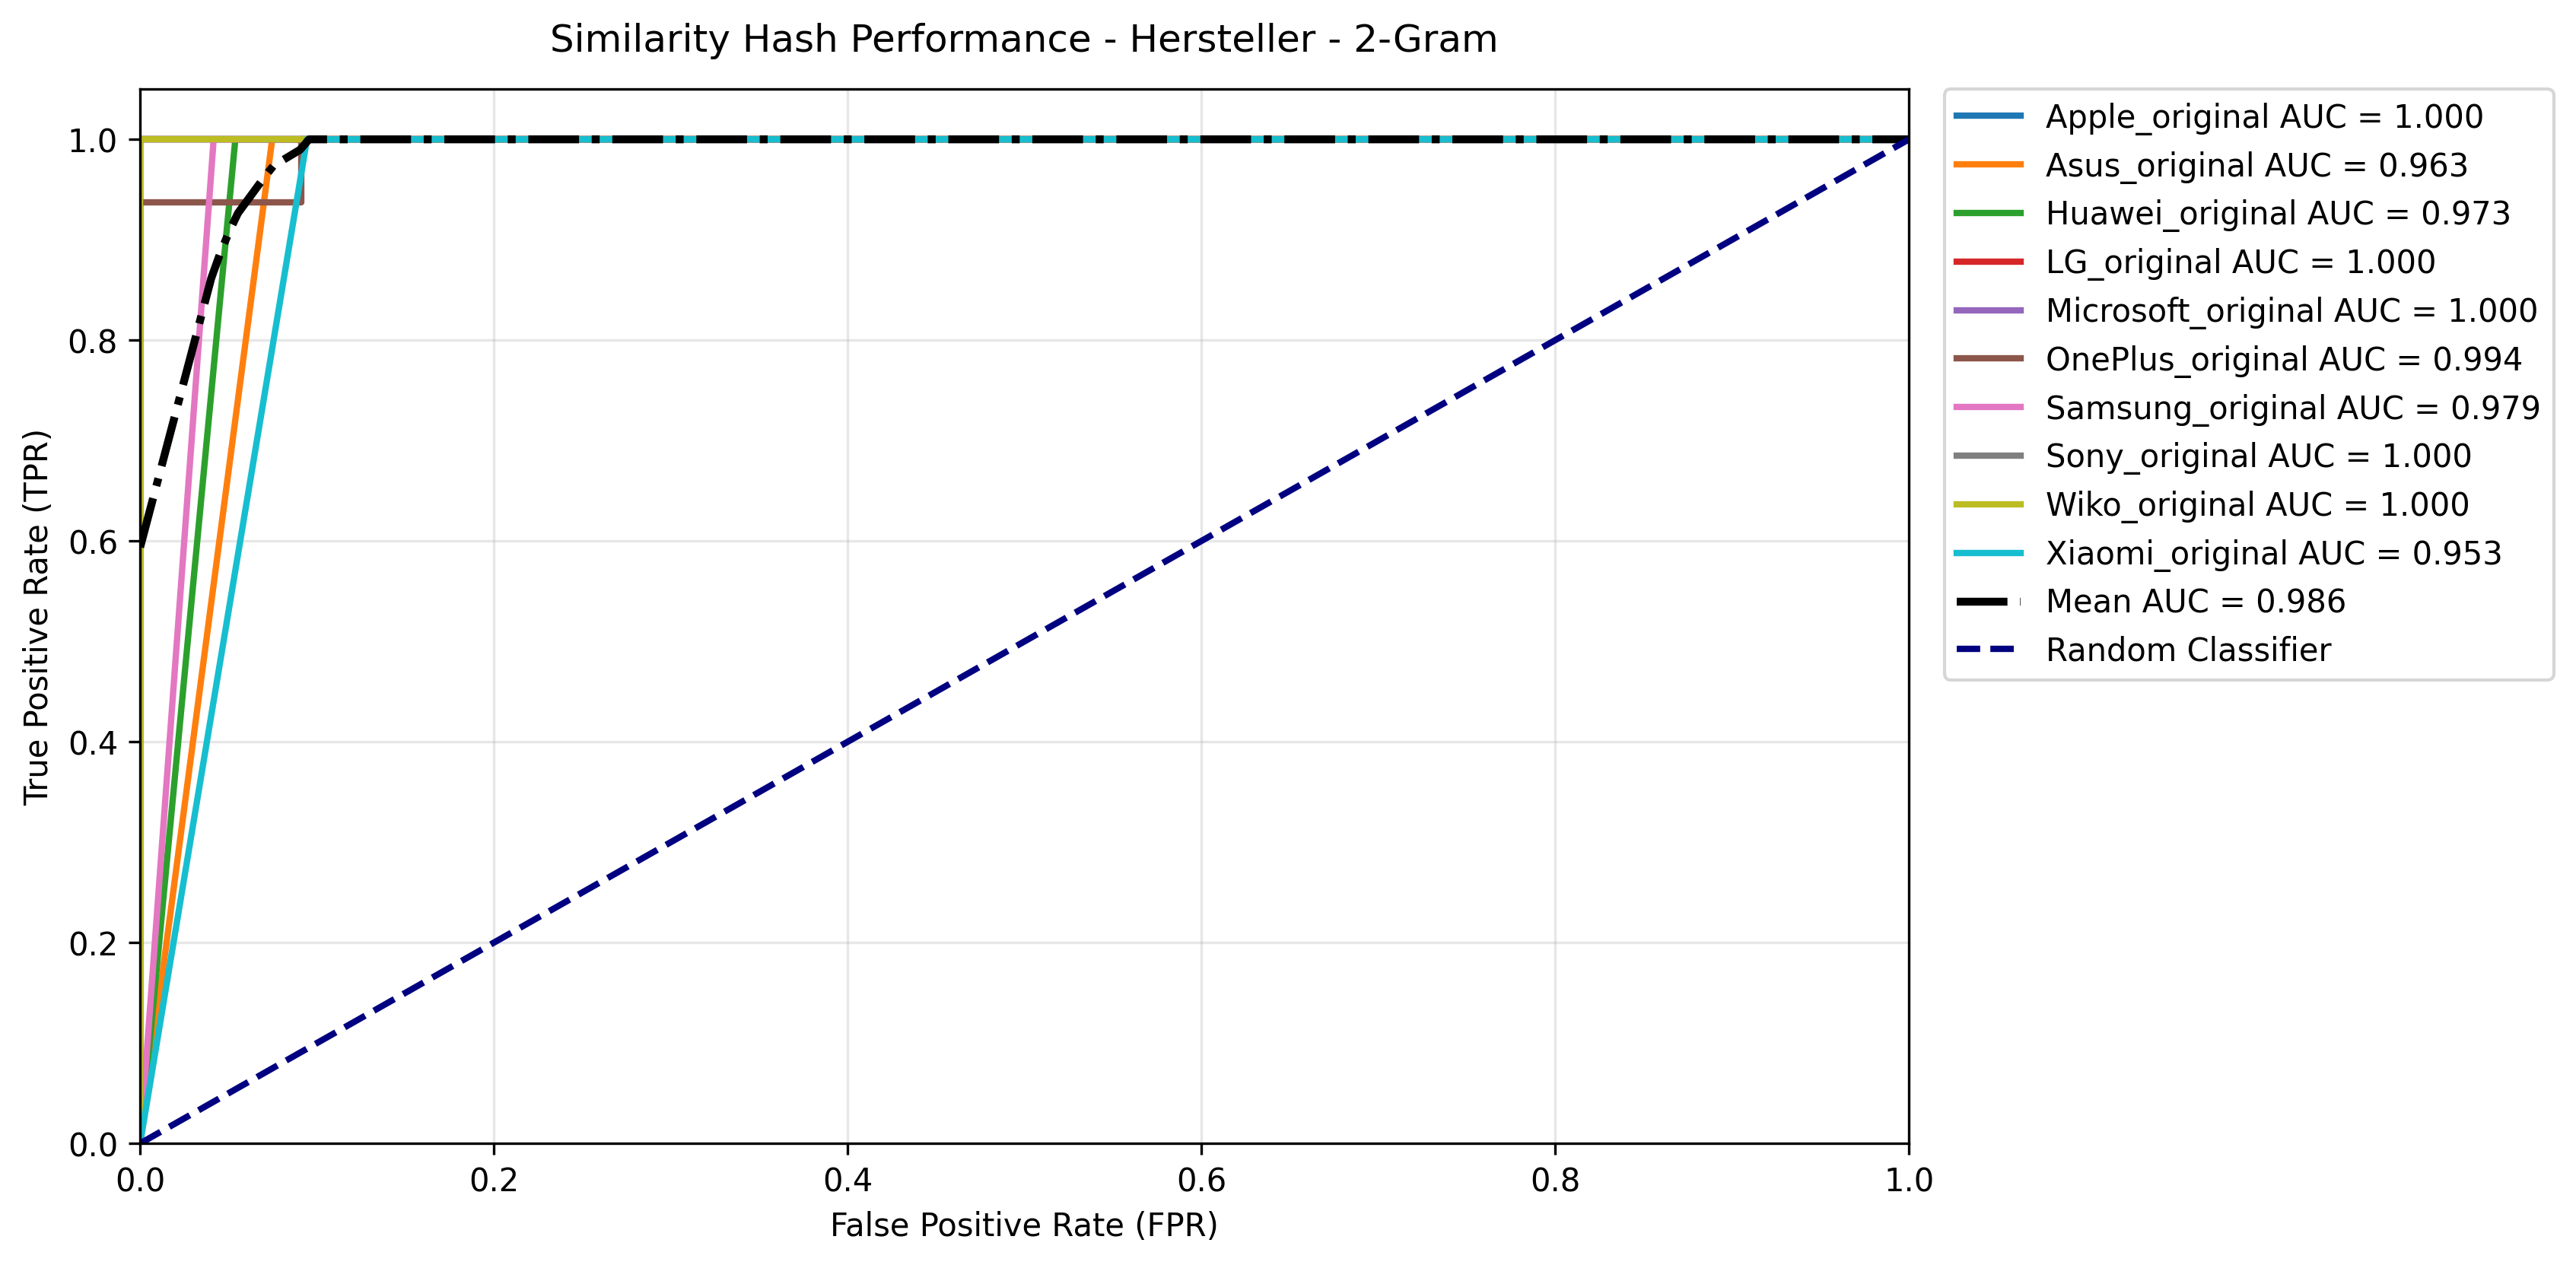
\includegraphics[width=1\linewidth]{grafiken/roc/brands.png}
    \caption{ROC-Analyse und AUC-Werte zur Quellkamera-Identifikation (SCI) auf Hersteller-Ebene mittels 2-Gramm-Similarity-Hashing (VISION-Datensatz)}
    \label{fig:auc_hersteller}
\end{figure}

\begin{figure}[!h]
    \centering
    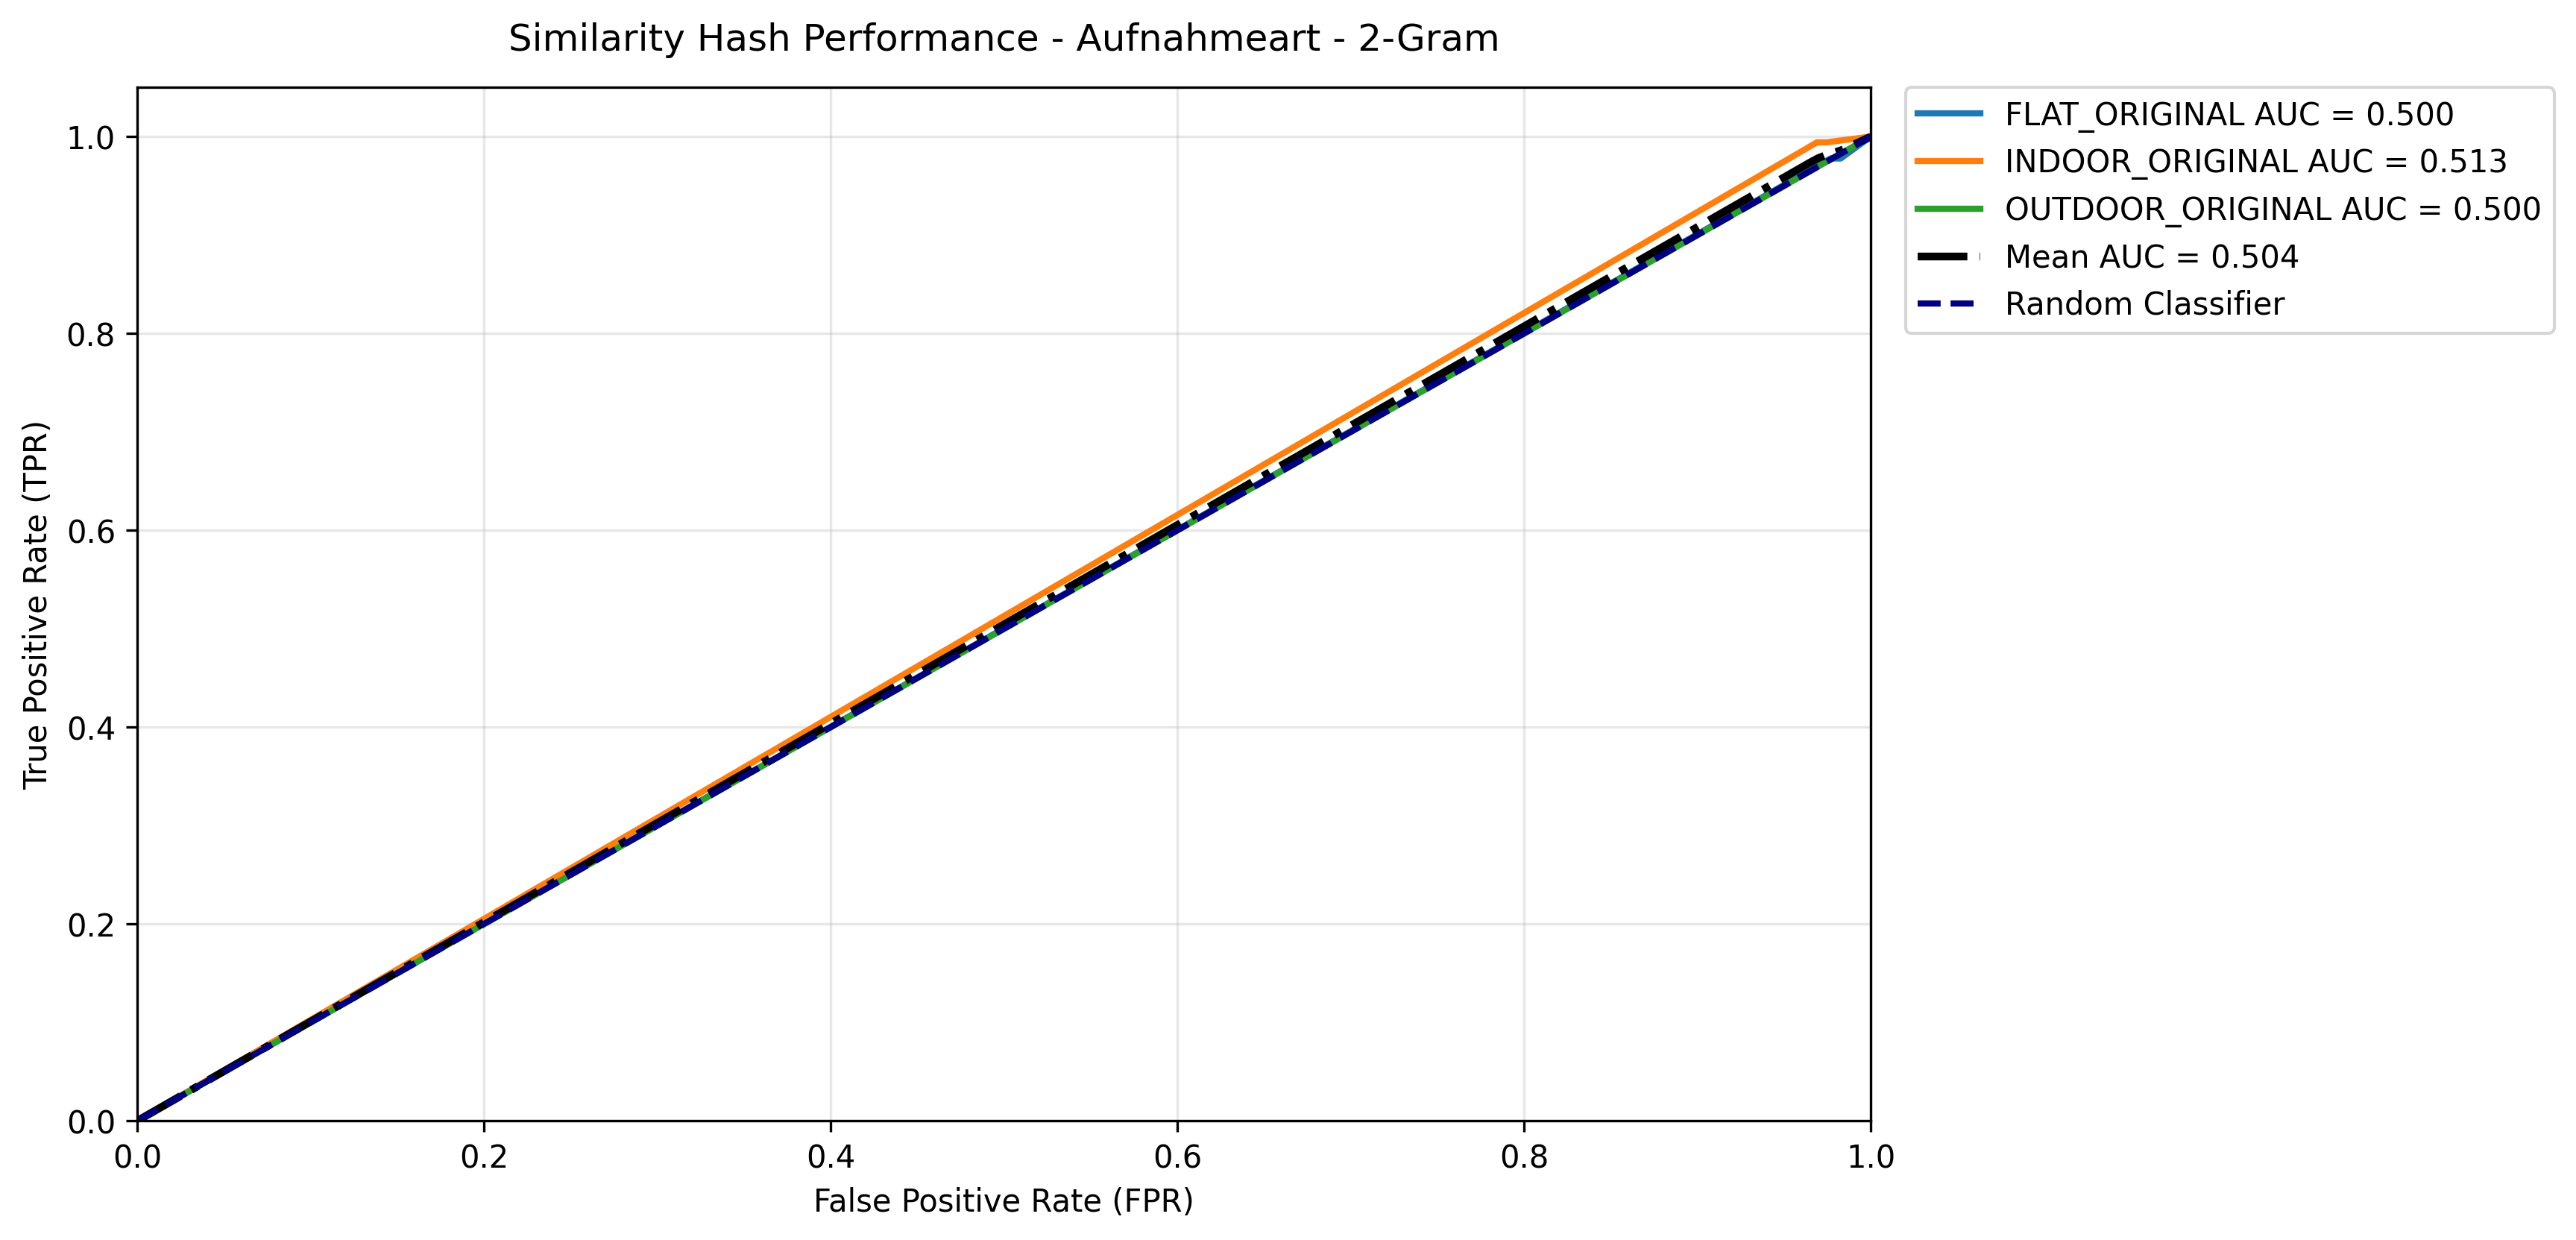
\includegraphics[width=1\linewidth]{grafiken/roc/contenttype.png}
    \caption{ROC-Analyse und AUC-Werte zur Quellkamera-Identifikation (SCI) auf Ebene der Aufnahmeart mittels 2-Gramm-Similarity-Hashing (VISION-Datensatz)}
    \label{fig:auc_aufnahmeart}
\end{figure}

Die Evaluation auf Ebene der individuellen physischen Endgeräte (siehe \cref{fig:auc_geraete}) erzielt einen durchschnittlichen AUC-Wert von 0.977. Eine detaillierte Betrachtung der strukturellen Ähnlichkeiten offenbart jedoch singuläre Herausforderungen bei der Differenzierung nah verwandter Geräte desselben Herstellers. Exemplarisch ist hierbei das Gerät D32 (OnePlus A3003) anzuführen, welches mit dem Gerät D25 (OnePlus A3000) eine berechnete Ähnlichkeit (Similarity) von 1,0 aufweist, obgleich der Digest von D32 aus vier zusätzlichen 2-Grammen konstituiert wird. Diese maximale Ähnlichkeitsbewertung verdeutlicht, dass die Container-Grammatik innerhalb einer eng verwandten Hardware-Generation oftmals eine so weitreichende Schnittmenge aufweist, dass das Fehlen einer Bestrafung für zusätzliche Boxen im asymmetrischen Tversky-Index zu vereinzelten falsch-positiven Zuordnungen führt.

% Modell

Bei der Klassifikation der spezifischen Gerätemodelle (siehe \cref{fig:auc_modell}) wird eine vergleichbare Trennschärfe mit einem AUC von 0.974 gemessen. Eine signifikante Anomalie stellt in dieser Untersuchungskategorie abermals das Modell OnePlus A3003 (D32) dar, welches ungewöhnlich hohe Falsch-Positiv-Raten in Bezug auf ausgewählte Samsung-Modelle (Ähnlichkeitswert von 0.933) sowie Huawei-Modelle (0.970) generiert. Dies ist auf die Nutzung weitgehend identischer Hardware-Encoder sowie auf Standard-Implementierungen innerhalb des Android-Media-Frameworks zurückzuführen, welche über Herstellergrenzen hinweg dieselbe Container-Grammatik erzeugen \cite{yang_comprehensive_2025}. Eine versuchsweise Erhöhung der n-Gramm-Länge auf n=4 senkt die absoluten Ähnlichkeitswerte in diesen spezifischen Fehlerfällen zwar leicht auf 0.921 respektive 0.823 ab, kann die zugrundeliegende strukturelle Gleichheit der Android-Basisarchitekturen jedoch nicht vollständig auflösen.

% Hersteller

Die Aggregation der Metadaten auf Hersteller-Ebene (siehe \cref{fig:auc_hersteller}) resultiert in der höchsten Klassifikationsleistung dieser Versuchsreihe mit einem AUC von 0.986. Insbesondere die Marken Apple, Microsoft, LG, Sony und Wiko lassen sich strukturell exzellent differenzieren und erreichen fehlerfreie Erkennungsraten. Diese Präzision begründet sich durch herstellerspezifische Besonderheiten in der Container-Architektur. Apple nutzt extensiv proprietäre QuickTime-Atome, Microsoft integriert spezifische Windows-Metadaten-Container und LG verwendet gesonderte Container zur Authentifizierung. Einen architektonischen Kontrast bildet Sony, dessen Geräte den minimalistischsten Container im gesamten Datensatz erzeugen und lediglich 25 unterschiedliche 2-Gramme aufweisen. Eine bemerkenswerte forensische Ausnahme stellt zudem der Hersteller Wiko dar. Die Marke integriert kein einziges proprietäres oder herstellerexklusives 2-Gramm, weshalb die 100-prozentige Erkennungsrate ausschließlich durch eine im Datensatz absolut einzigartige Anordnung (Topologie) der Standard-Atome erreicht wird.

% Aufnahmeart

Abschließend wird die Trennschärfe hinsichtlich der physikalischen Aufnahmeart (Flat, Indoor, Outdoor) evaluiert (siehe \cref{fig:auc_aufnahmeart}). Wie mit einem AUC von 0.504 zu erwarten, bildet das Verfahren hierbei lediglich eine Gleichverteilung nach. Abgesehen von den Geräten D24 (Xiaomi RedmiNote3) und D32 (OnePlus A3003), welche in Abhängigkeit des Content-Types eine leicht modifizierte Containerstruktur generierten, konnten keine messbaren Differenzen bei den extrahierten n-Grammen nach Aufnahmeumgebung nachgewiesen werden. Dieses Resultat ist methodisch zwingend plausibel, da bei der Erstellung des VISION-Datensatzes keine veränderten manuellen Kameraeinstellungen je nach Content-Type vorgenommen wurden \cite[Kap. 3]{shullani_vision_2017}. Folglich hinterlässt die physische Umgebung keine Spuren in der Syntax des MP4-Containers.

%%%

\subsection{Social-Media-Videos}

Dieser Abschnitt evaluiert die Zuverlässigkeit des Verfahrens im Kontext der Plattform-Erkennung (SNA, Social Network Attribution). Der Upload von Videodateien auf Social-Media-Plattformen (\cref{fig:auc_sm}) führt in der Regel zum Verlust der nativen Container-Signatur, da die Dateien auf den Servern neu verarbeitet werden und in eine plattformspezifische Baumstruktur überführt werden. Um nachzuweisen, dass das Similarity Hashing diese Distributionsplattformen dennoch zuverlässig klassifizieren kann, werden die Testdaten nach den jeweiligen Plattformen (z. B. YouTube, WhatsApp, Facebook, TikTok) und nativen Aufnahmen gefiltert. Die nachträglich veränderten Videos, die außerdem in der Eva-Datenbank vorhanden sind, wurden explizit ausgeschlossen. Der Source-Digest wird hierbei isoliert für den jeweiligen Verarbeitungstyp der Social-Media-Plattform gebildet, ungeachtet der ursprünglichen Kamera, um die rein plattformspezifische Container-Grammatik zu abstrahieren.\\

\begin{figure}[h]
    \centering
    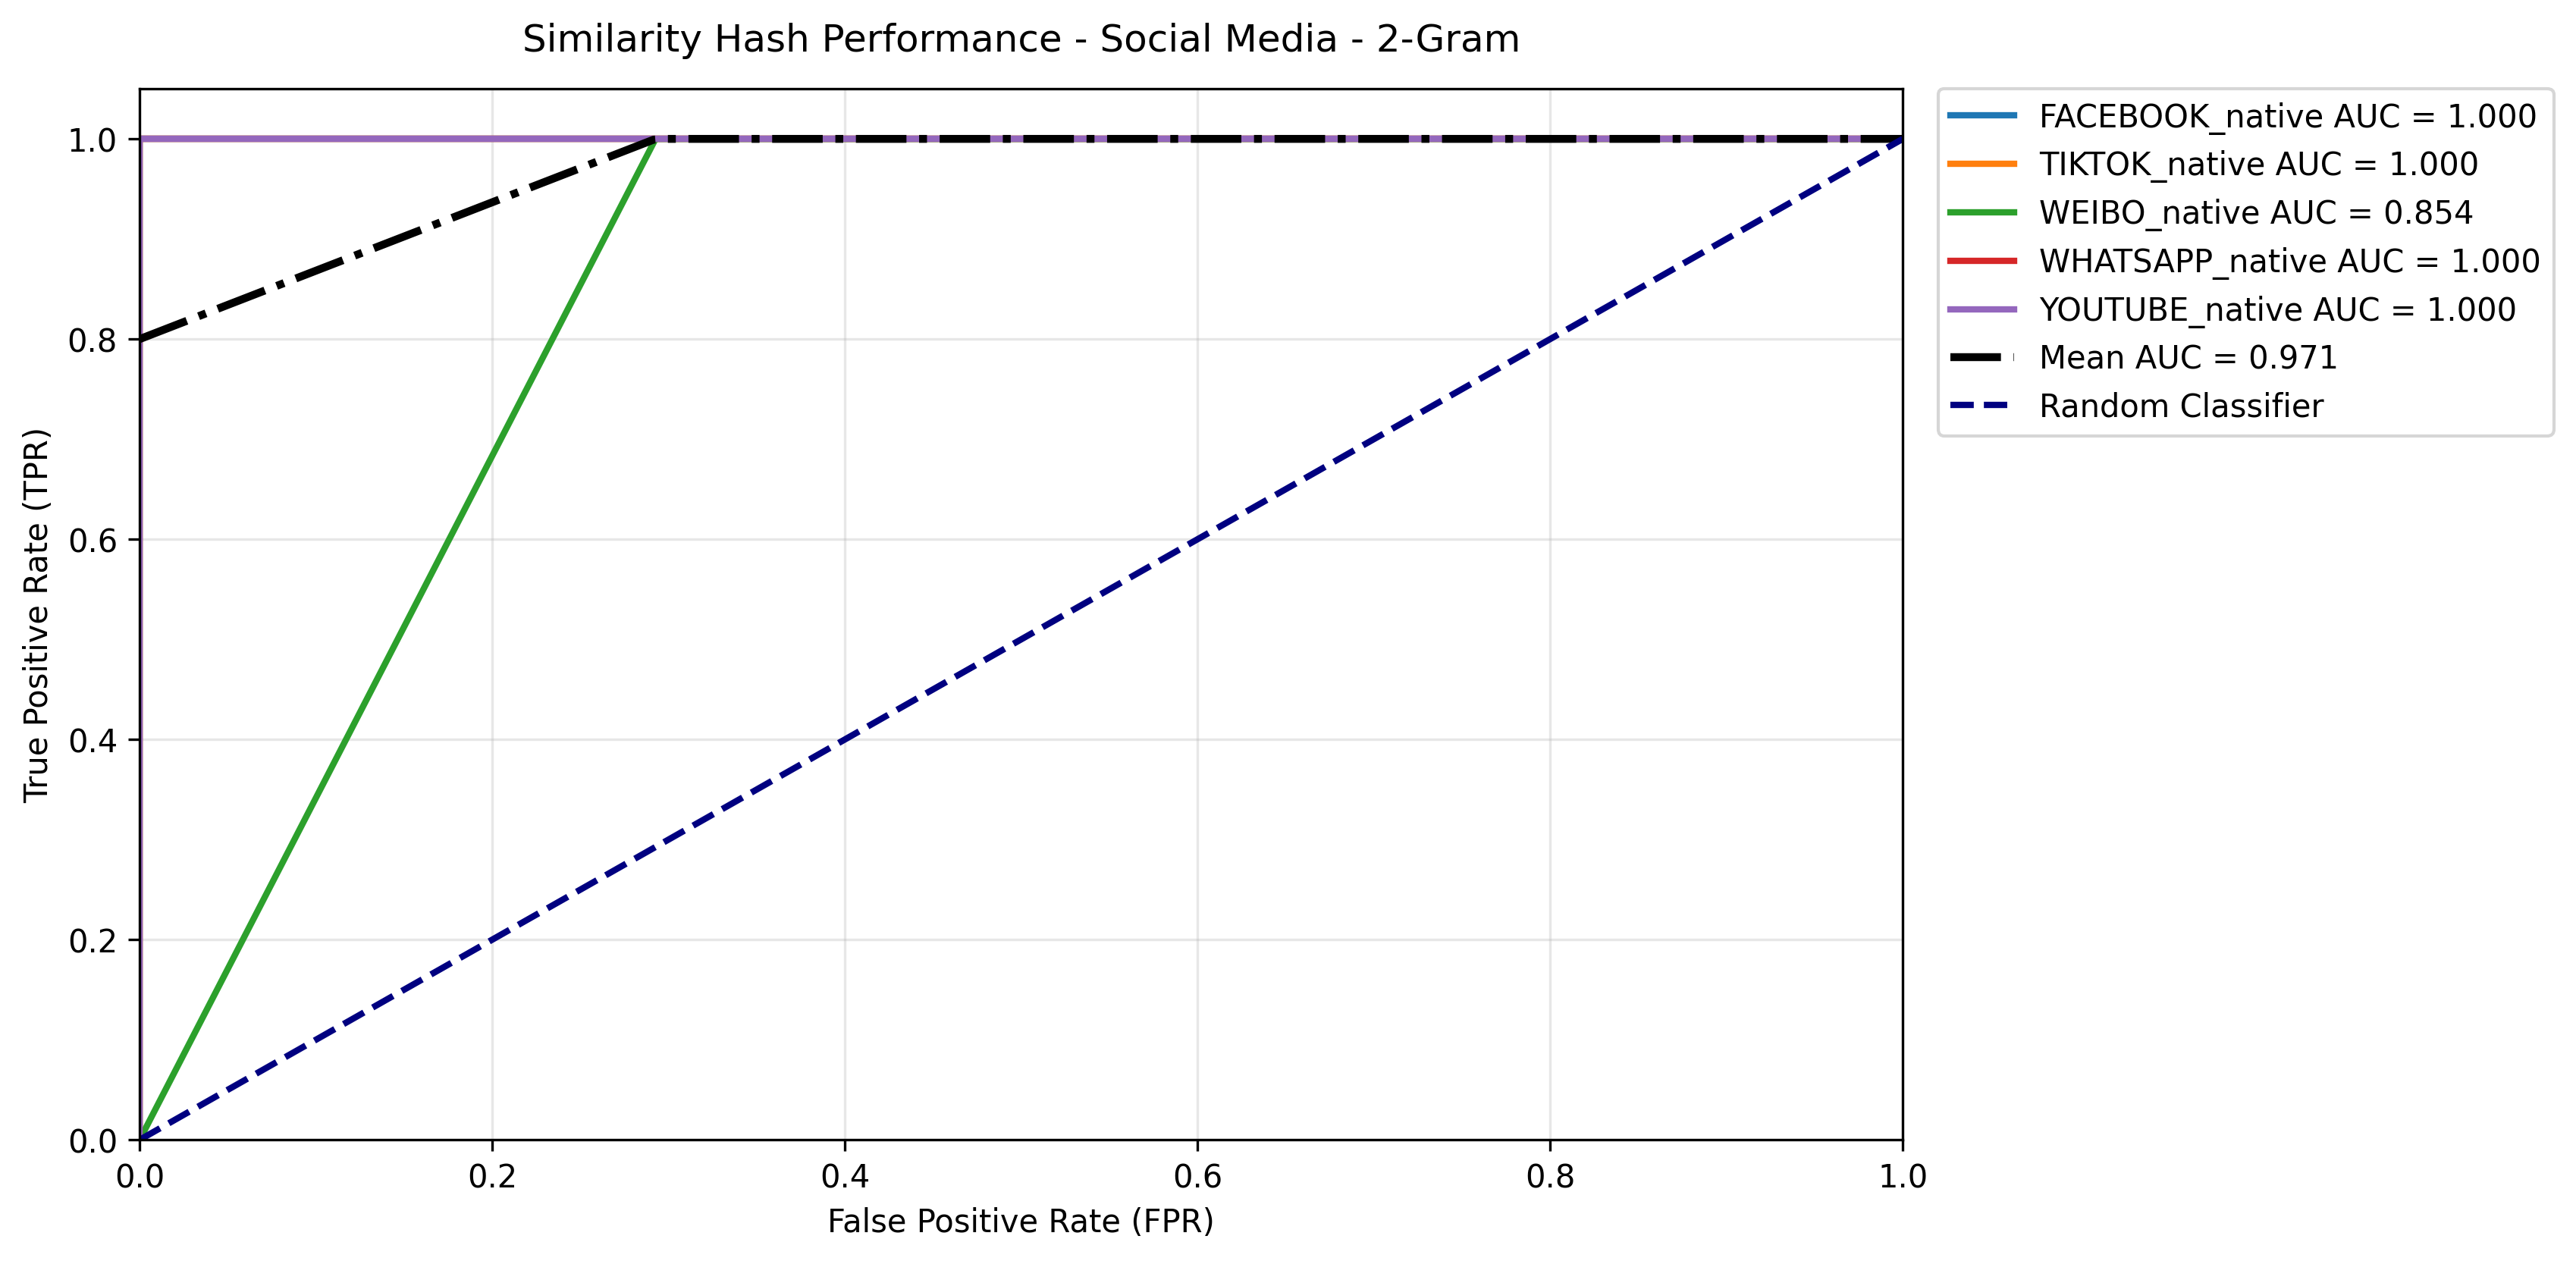
\includegraphics[width=1\linewidth]{grafiken/roc/sm2.png}
    \caption{ROC-Analyse und AUC-Werte zur Zuordnung zu Social-Media-Plattformen (SNA) mittels 2-Gramm-Similarity-Hashing (Vision- und EVA-7K-Datensatz)}
    \label{fig:auc_sm}
\end{figure}

Die Auswertung der Klassifikationsleistung zur Zuordnung zu sozialen Netzwerken (siehe \cref{fig:auc_sm}) weist eine Trennschärfe mit AUC-Wert von 0.971 aus. Insbesondere für die Plattformen Facebook, TikTok, WhatsApp und YouTube wird eine fehlerfreie Erkennungsrate von 1.000 erzielt. Diese hohe Präzision resultiert aus der serverseitigen Transkodierung der Netzwerke, bei der die nativen Strukturen verworfen und in eine plattformspezifische Baumstruktur überführt werden \cite[Kap. 5.4.4]{yang_comprehensive_2025}. Die strukturelle Analyse zeigt, dass die extrahierte n-Gramm-Struktur für TikTok geräteübergreifend vollständig identisch ist. Ein vergleichbares Verhalten ist bei WhatsApp, YouTube und Facebook zu erkennen. Bei diesen Plattformen liegt nach der Verarbeitung eine geräteübergreifend identische Reihenfolge der Container-Boxen vor, welche sich lediglich durch das Vorhandensein einzelner, abweichender Container unterscheidet \cite[Kap. 4]{yang_efficient_2020}. Die Stringenz dieser Standardisierung der Plattform-Encoder wird zusätzlich dadurch belegt, dass selbst bei dem nativ ausgeschlossenen Gerät Lenovo P70-A (D07) in den zugehörigen Social-Media-Derivaten keine Auffälligkeiten in der Struktur der n-Gramme erkannt werden konnten.

Eine signifikante Abweichung von dieser Homogenisierung weist die Plattform Weibo auf, welche mit einem AUC-Wert von 0.854 eine messbar geringere Klassifikationsleistung verzeichnet. Im Kontrast zu den übrigen Netzwerken enthalten Weibo-Derivate weiterhin stark variierende Containerstrukturen. Da die native Architektur bei der serverseitigen Verarbeitung durch diese Plattform nicht vollständig überschrieben wird, bleiben strukturelle Varianzen erhalten, welche weiterhin direkte Rückschlüsse auf das ursprüngliche Aufnahmegerät zulassen und somit eine rein plattformspezifische Klassifikation erschweren \cite[Kap. 5]{xiang_forensic_2021}.

%%%

\subsection{Synthetische Videos}

In dieser Kategorie verlagert sich die forensische Quellenerkennung von physischer Hardware auf rein softwarebasierte Generatoren. Evaluiert wird, ob vollständig durch Image-to- und Text-to-Video-Modelle (\cref{fig:auc_ai} und \ref{fig:auc_dfsynth}) generierte Inhalte aus dem eigens erstellten KI-Datensatz verlässlich identifiziert werden können. Analog zur Gerätekennung werden Source-Digests für die spezifischen KI-Modelle generiert. Der Fokus der Untersuchung liegt darauf, ob generative KI-Modelle eine hinreichend spezifische syntaktische Signatur hinterlassen. Dies betrifft insbesondere die Integration proprietärer Metadaten oder kryptografischer Manifeste (wie C2PA-Signaturen), die typischerweise in der optionalen uuid-Box des Containers gespeichert werden und sich strukturell von nativen Aufnahmen abgrenzen lassen.\\

\begin{figure}[h]
    \centering
    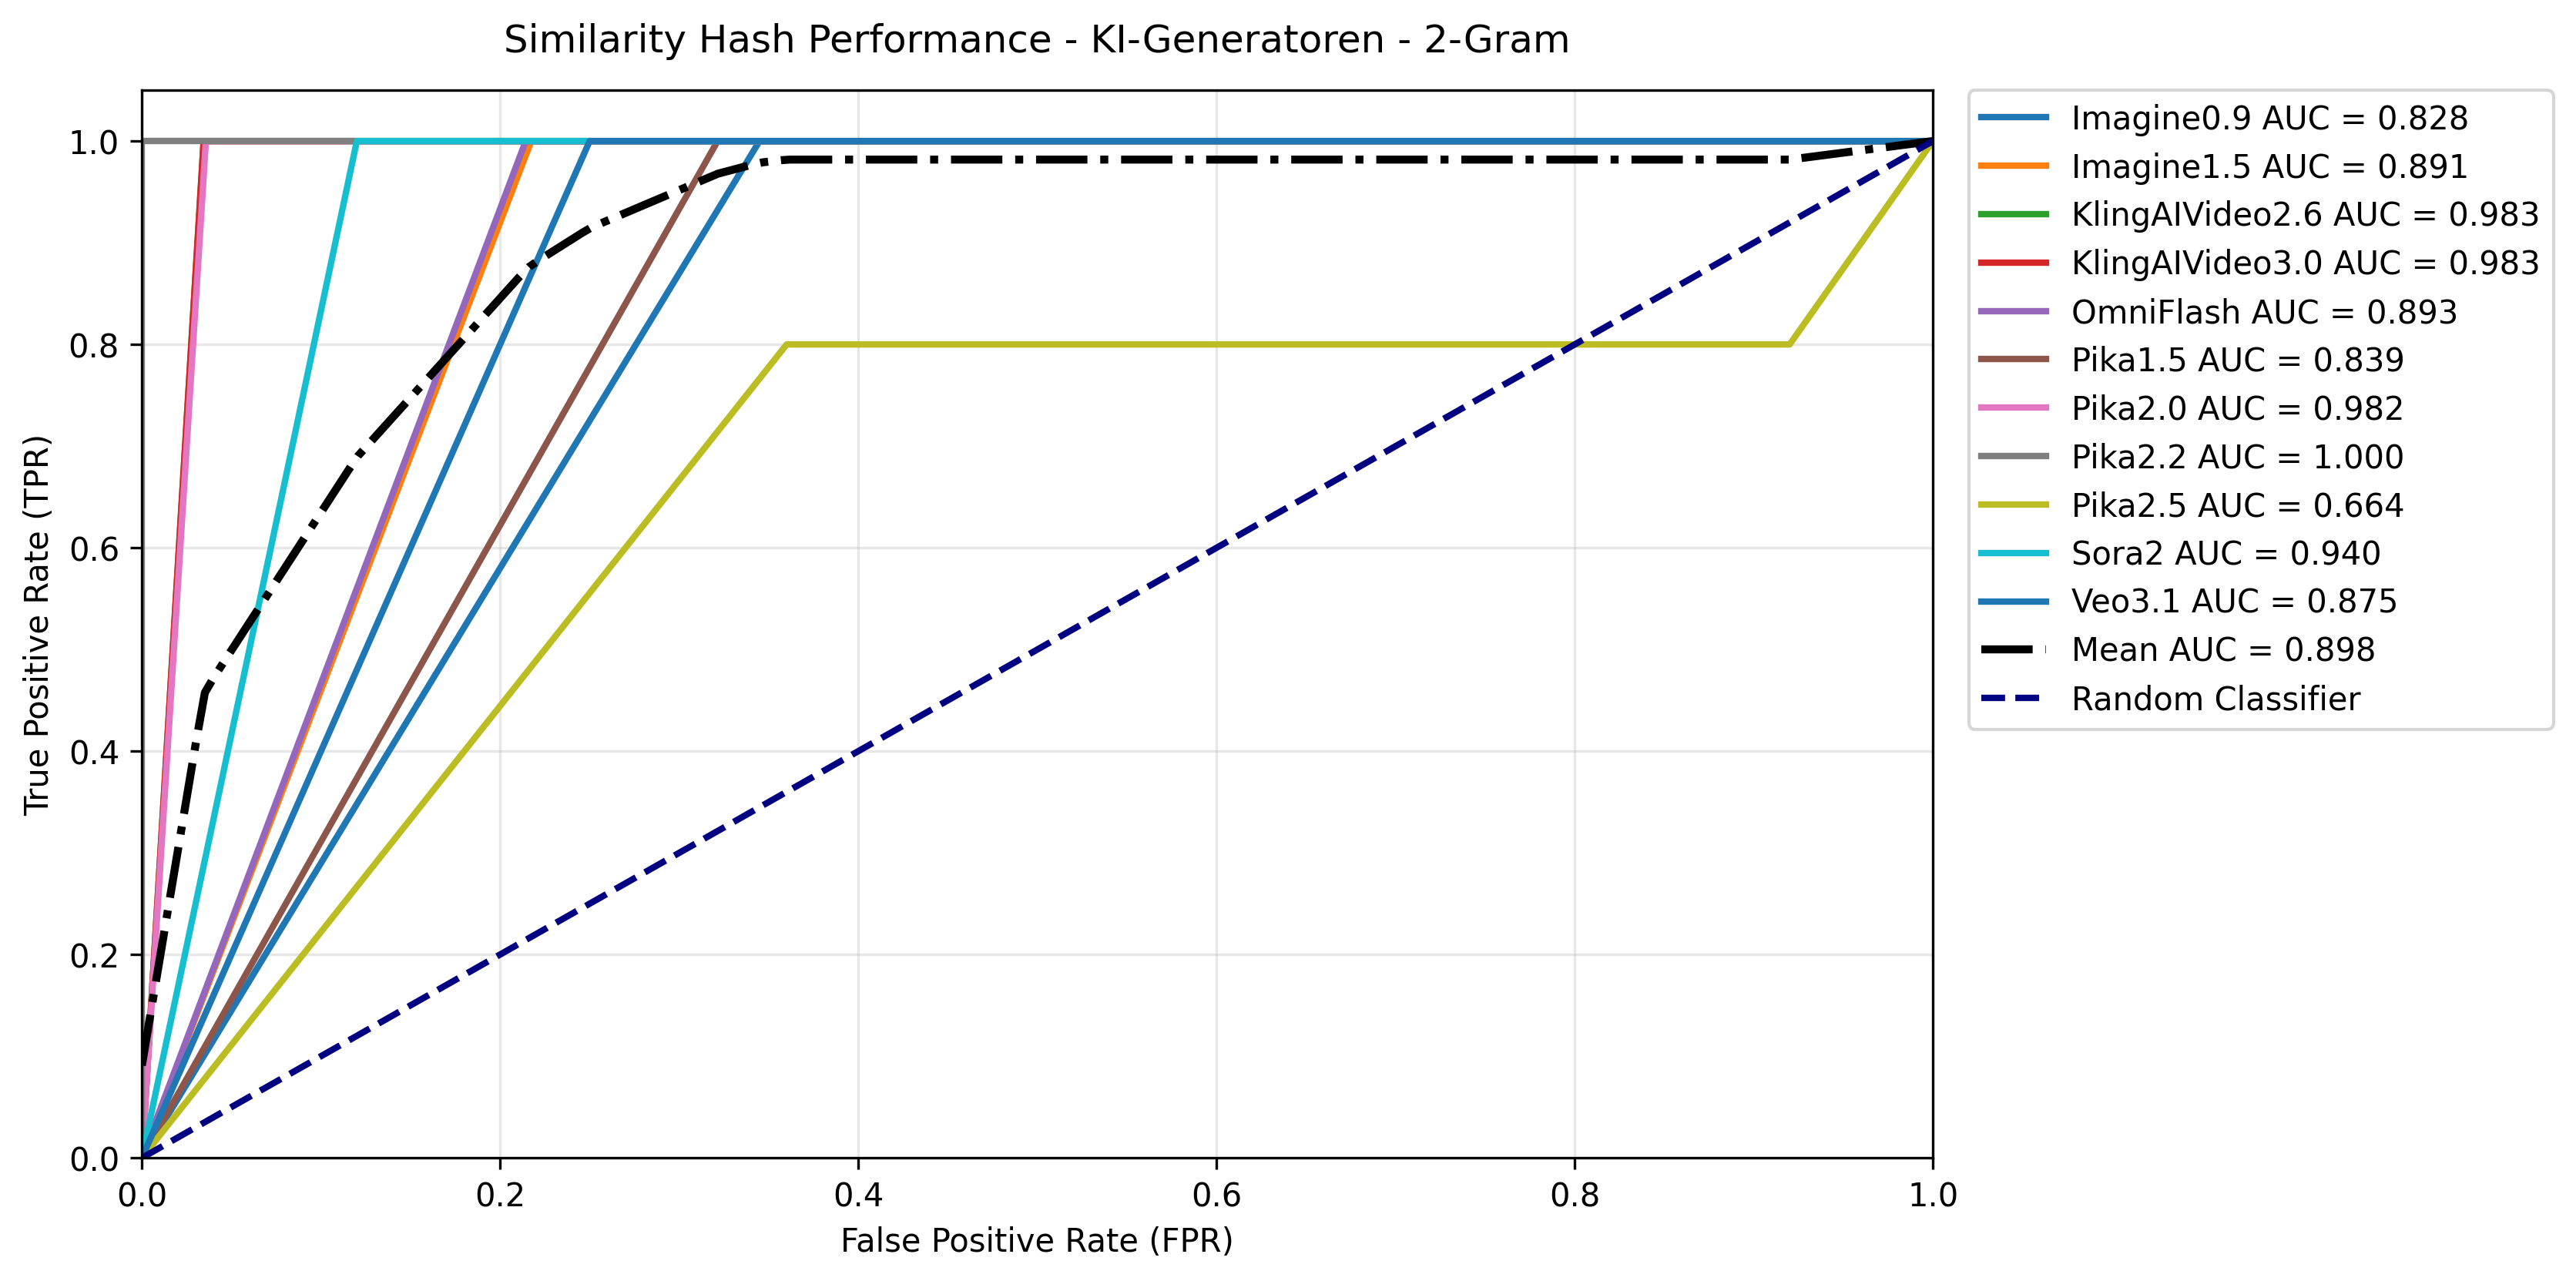
\includegraphics[width=1\linewidth]{grafiken/roc/ai.png}
    \caption{ROC-Analyse und AUC-Werte zur Identifikation von KI-Modellen mittels 2-Gramm-Similarity-Hashing (Eigener KI-Datensatz)}
    \label{fig:auc_ai}
\end{figure}

\begin{figure}[h]
    \centering
    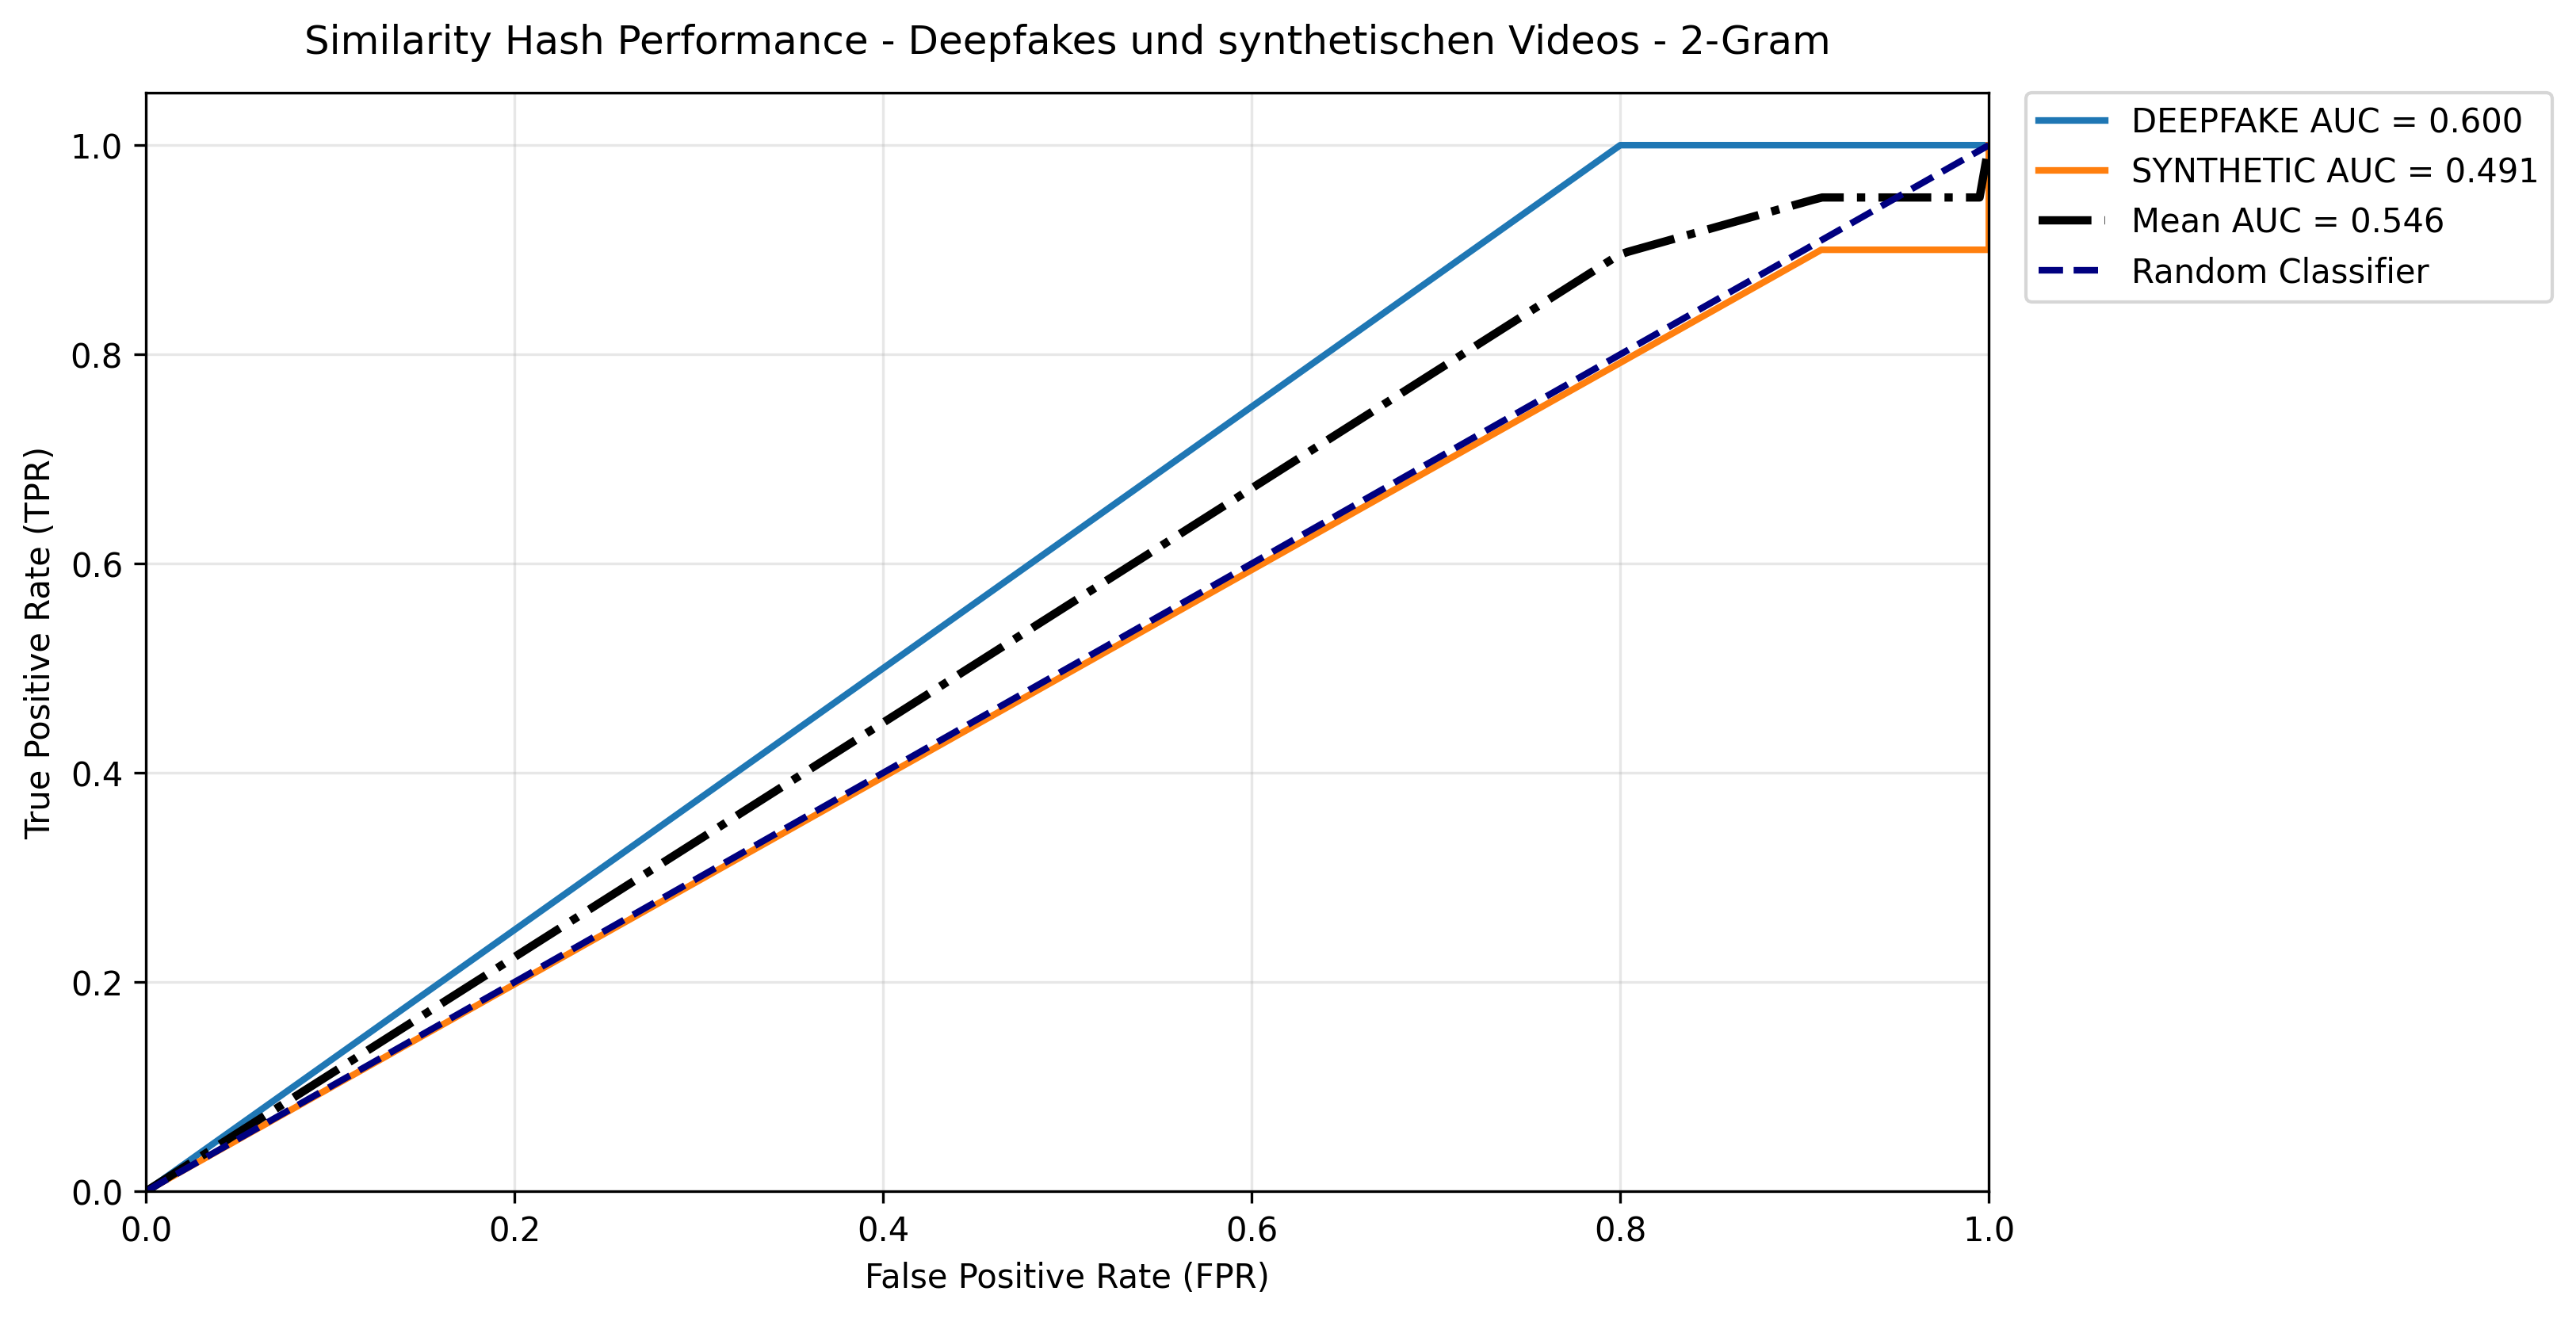
\includegraphics[width=1\linewidth]{grafiken/roc/dfsynth.png}
    \caption{ROC-Analyse und AUC-Werte zur unterscheidung von synthetischen Videos und Deepfakes mittels 2-Gramm-Similarity-Hashing (Eigener KI-Datensatz)}
    \label{fig:auc_dfsynth}
\end{figure}

% Model

Die Evaluation der spezifischen KI-Generatoren (siehe \cref{fig:auc_ai}) erzielt einen AUC-Wert von 0.898. Eine detaillierte Analyse der zugrundeliegenden Source Digests offenbart, dass sich die Identifikation primär auf spezifische Container-Boxen stützt, die bei nativen Smartphone-Aufnahmen nahezu nie in Erscheinung treten. Insbesondere zeichnet sich die Mehrheit der untersuchten KI-Modelle durch die Integration der Atome \(btrt\) (Bit Rate Box), \(sbgp\) (Sample-to-Group Box) sowie \(sgpd\) (Sample Group Description Box) aus, wodurch eine charakteristische KI-Signatur in der Metadaten-Topologie erzeugt wird. Die Auswertung zeigt jedoch auch signifikante strukturelle Inkonsistenzen innerhalb der Modellfamilien auf, was den durchschnittlichen Erkennungswert reduziert. So produzieren spezifische Generatoren, wie etwa die Ausprägungen Pika 2.0 und Pika 2.2, Container-Strukturen, die keine dieser eindeutigen Fremdatome aufweisen und sich stattdessen stark an der Grammatik nativer Aufnahmen orientieren. Diese strukturelle Unauffälligkeit erhöht das Risiko von falsch-positiven Zuordnungen bei diesen spezifischen Modellen.

% df synth

Die Differenzierung zwischen bild- als auch videobasierten Deepfakes und vollständig synthetisierten Text-to-Video-Inhalten (siehe \cref{fig:auc_dfsynth}) verzeichnet hingegen einen niedrigen AUC-Wert von lediglich 0.546. Um eine methodisch belastbare und symmetrische Vergleichsbasis zu gewährleisten, wurde diese Auswertung zwingend auf jene KI-Datensätze limitiert, in denen das jeweilige Modell sowohl Deepfakes als auch synthetische Repräsentationen zur Verfügung stellte (spezifisch die Modelle AI01, AI02, AI04, AI07 und AI11). Der gemessene AUC-Wert, welcher sich de facto einer stochastischen Gleichverteilung annähert, belegt, dass eine rein syntaktische Separation dieser beiden Erzeugungsarten auf Container-Ebene durch das 2-Gramm-Hashing nicht realisierbar ist. Daraus ist abzuleiten, dass die zugrundeliegenden KI-Plattformen unabhängig vom initialen Input identische, standardisierte Prozesse für die finale MP4-Generierung anwenden. Aus dieser Limitation resultiert für zukünftige Forschungsarbeiten (Future Work) die Notwendigkeit, zu evaluieren, ob jenseits der einfachen Container-Topologie alternative forensische Artefakte existieren, die eine verlässliche Unterscheidung zwischen synthetischen Inhalten und Deepfakes ermöglichen.

%%%

\subsection{Gemischte Videos}

Der abschließende Teil der kategorialen Auswertung (\cref{fig:auc_bearbeitungen} und \ref{fig:auc_mixed}) widmet sich der Identifikation von Manipulationssoftware (MTI) sowie der übergeordneten Klassifikation der drei primären Erzeugerquellen (native Aufnahmen, Social-Media-Derivate und KI-generierte Inhalte). Zur Evaluation der Bearbeitungssoftware dienen modifizierte EVA-7K-Videos als Testdaten, welche gegen neun softwarespezifische Source Digests klassifiziert werden. Die übergeordnete Separation der drei primären Erzeugerkategorien, mit jeweils einem Source Digest über jede Kategorie hinweg, wurde hingegen nur auf unveränderten Videos der Vision- und EVA-7K-Datensätze durchgeführt.

\begin{figure}[h]
    \centering
    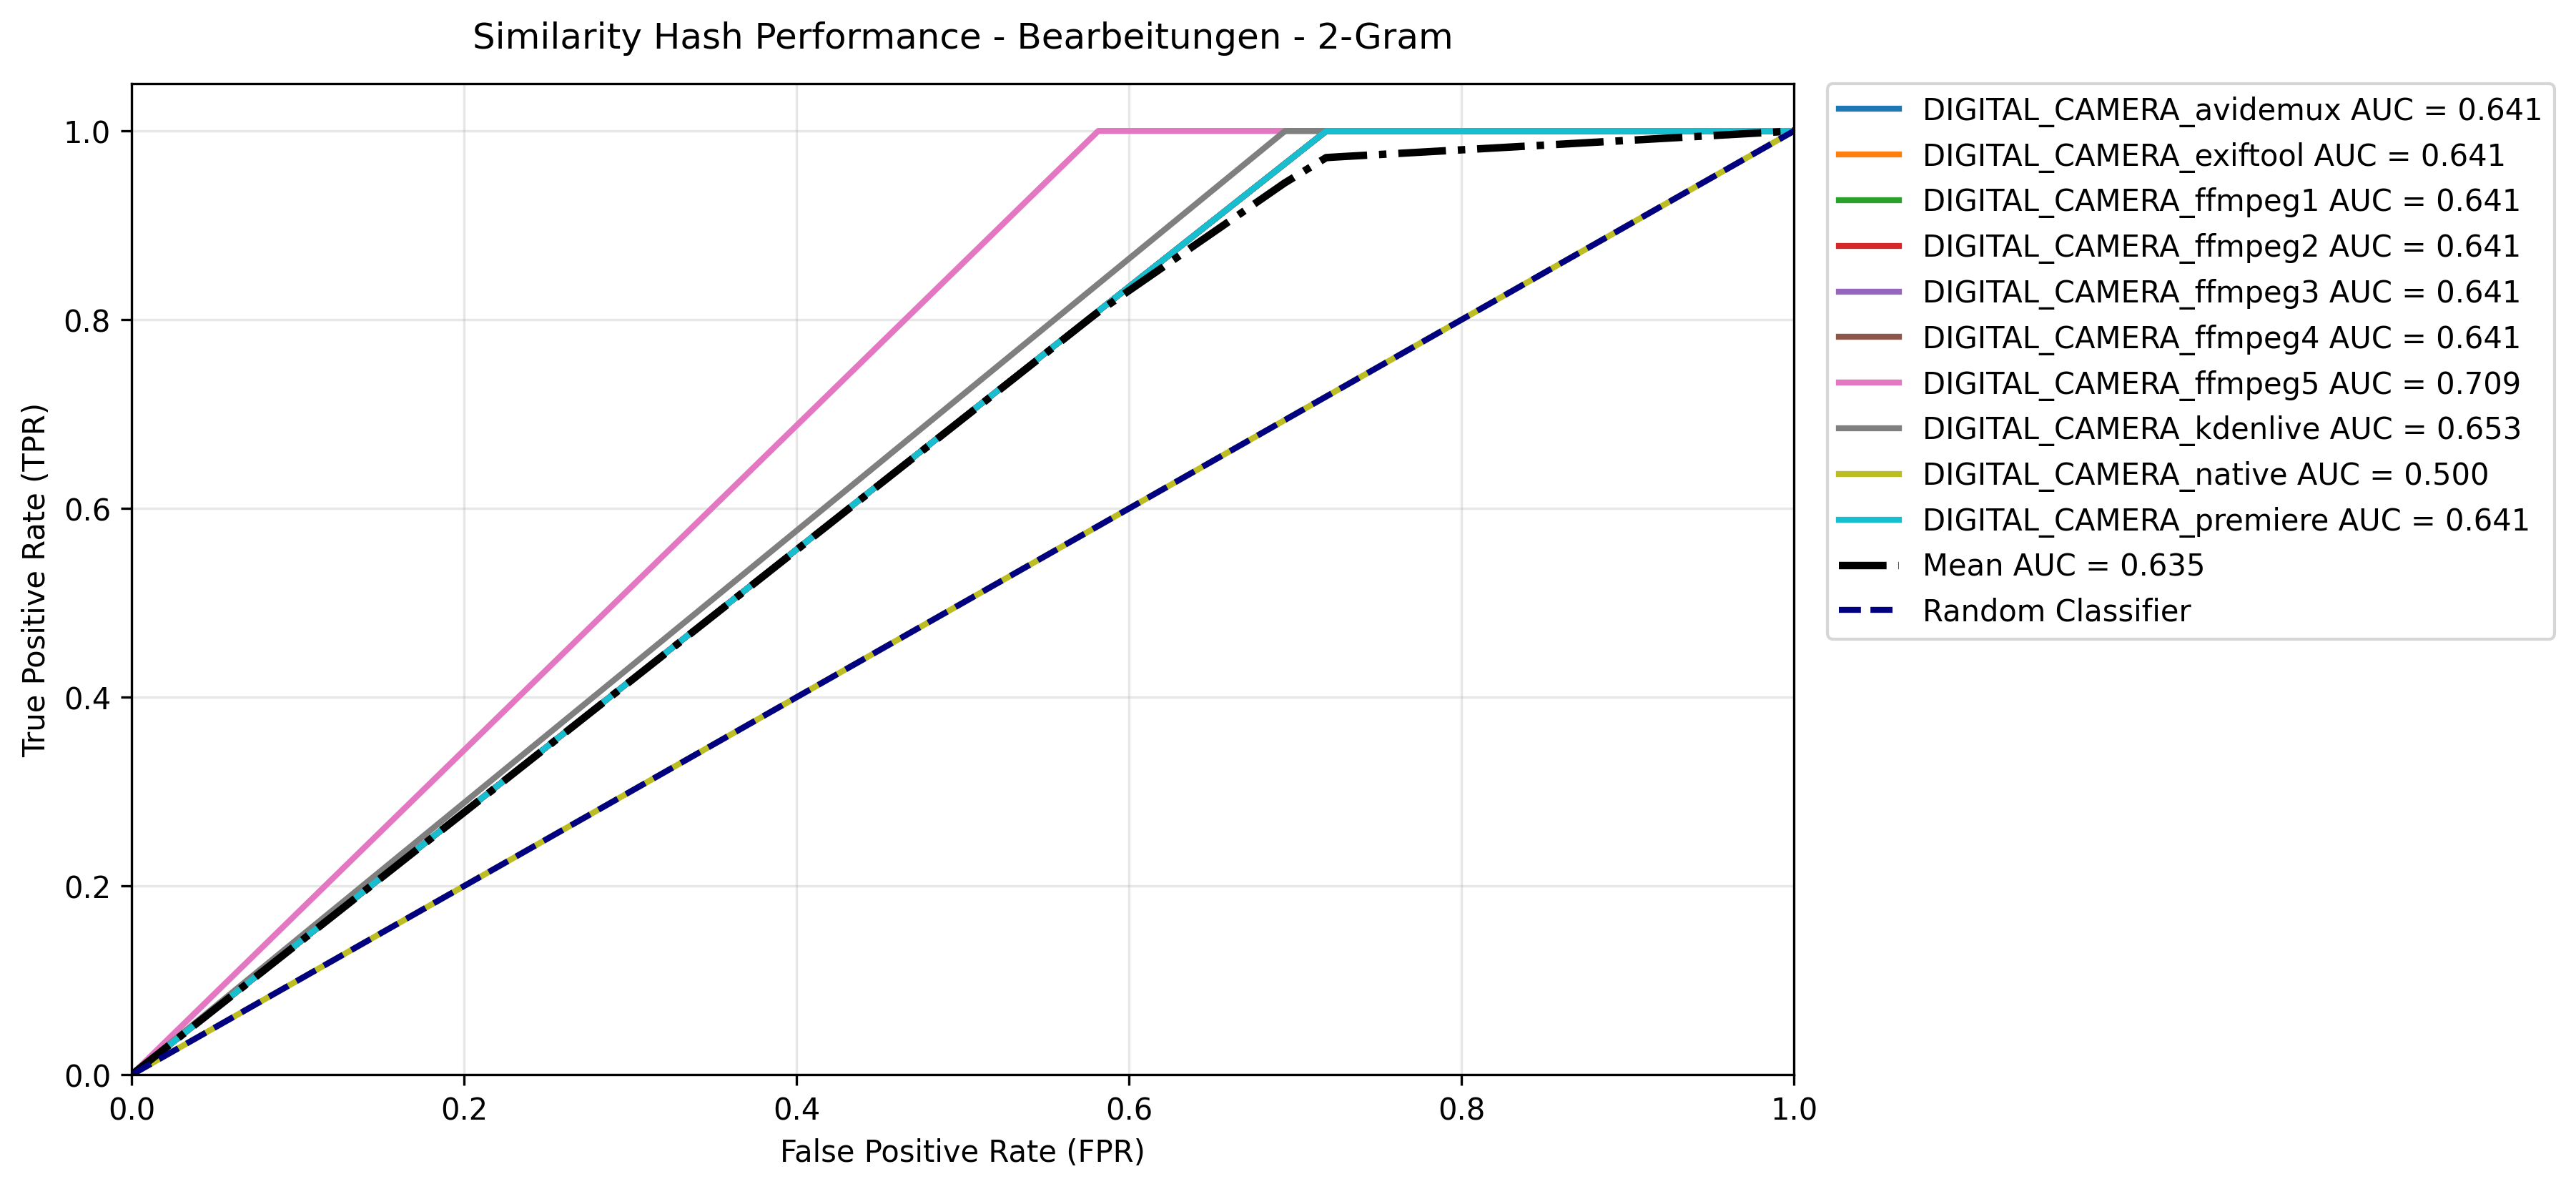
\includegraphics[width=1\linewidth]{grafiken/roc/tampered.png}
    \caption{ROC-Analyse und AUC-Werte zur Identifikation der Bearbeitungssoftware (MTI) mittels 2-Gramm-Similarity-Hashing (EVA-7K-Datensatz)}
    \label{fig:auc_bearbeitungen}
\end{figure}


\begin{figure}[!h]
    \centering
    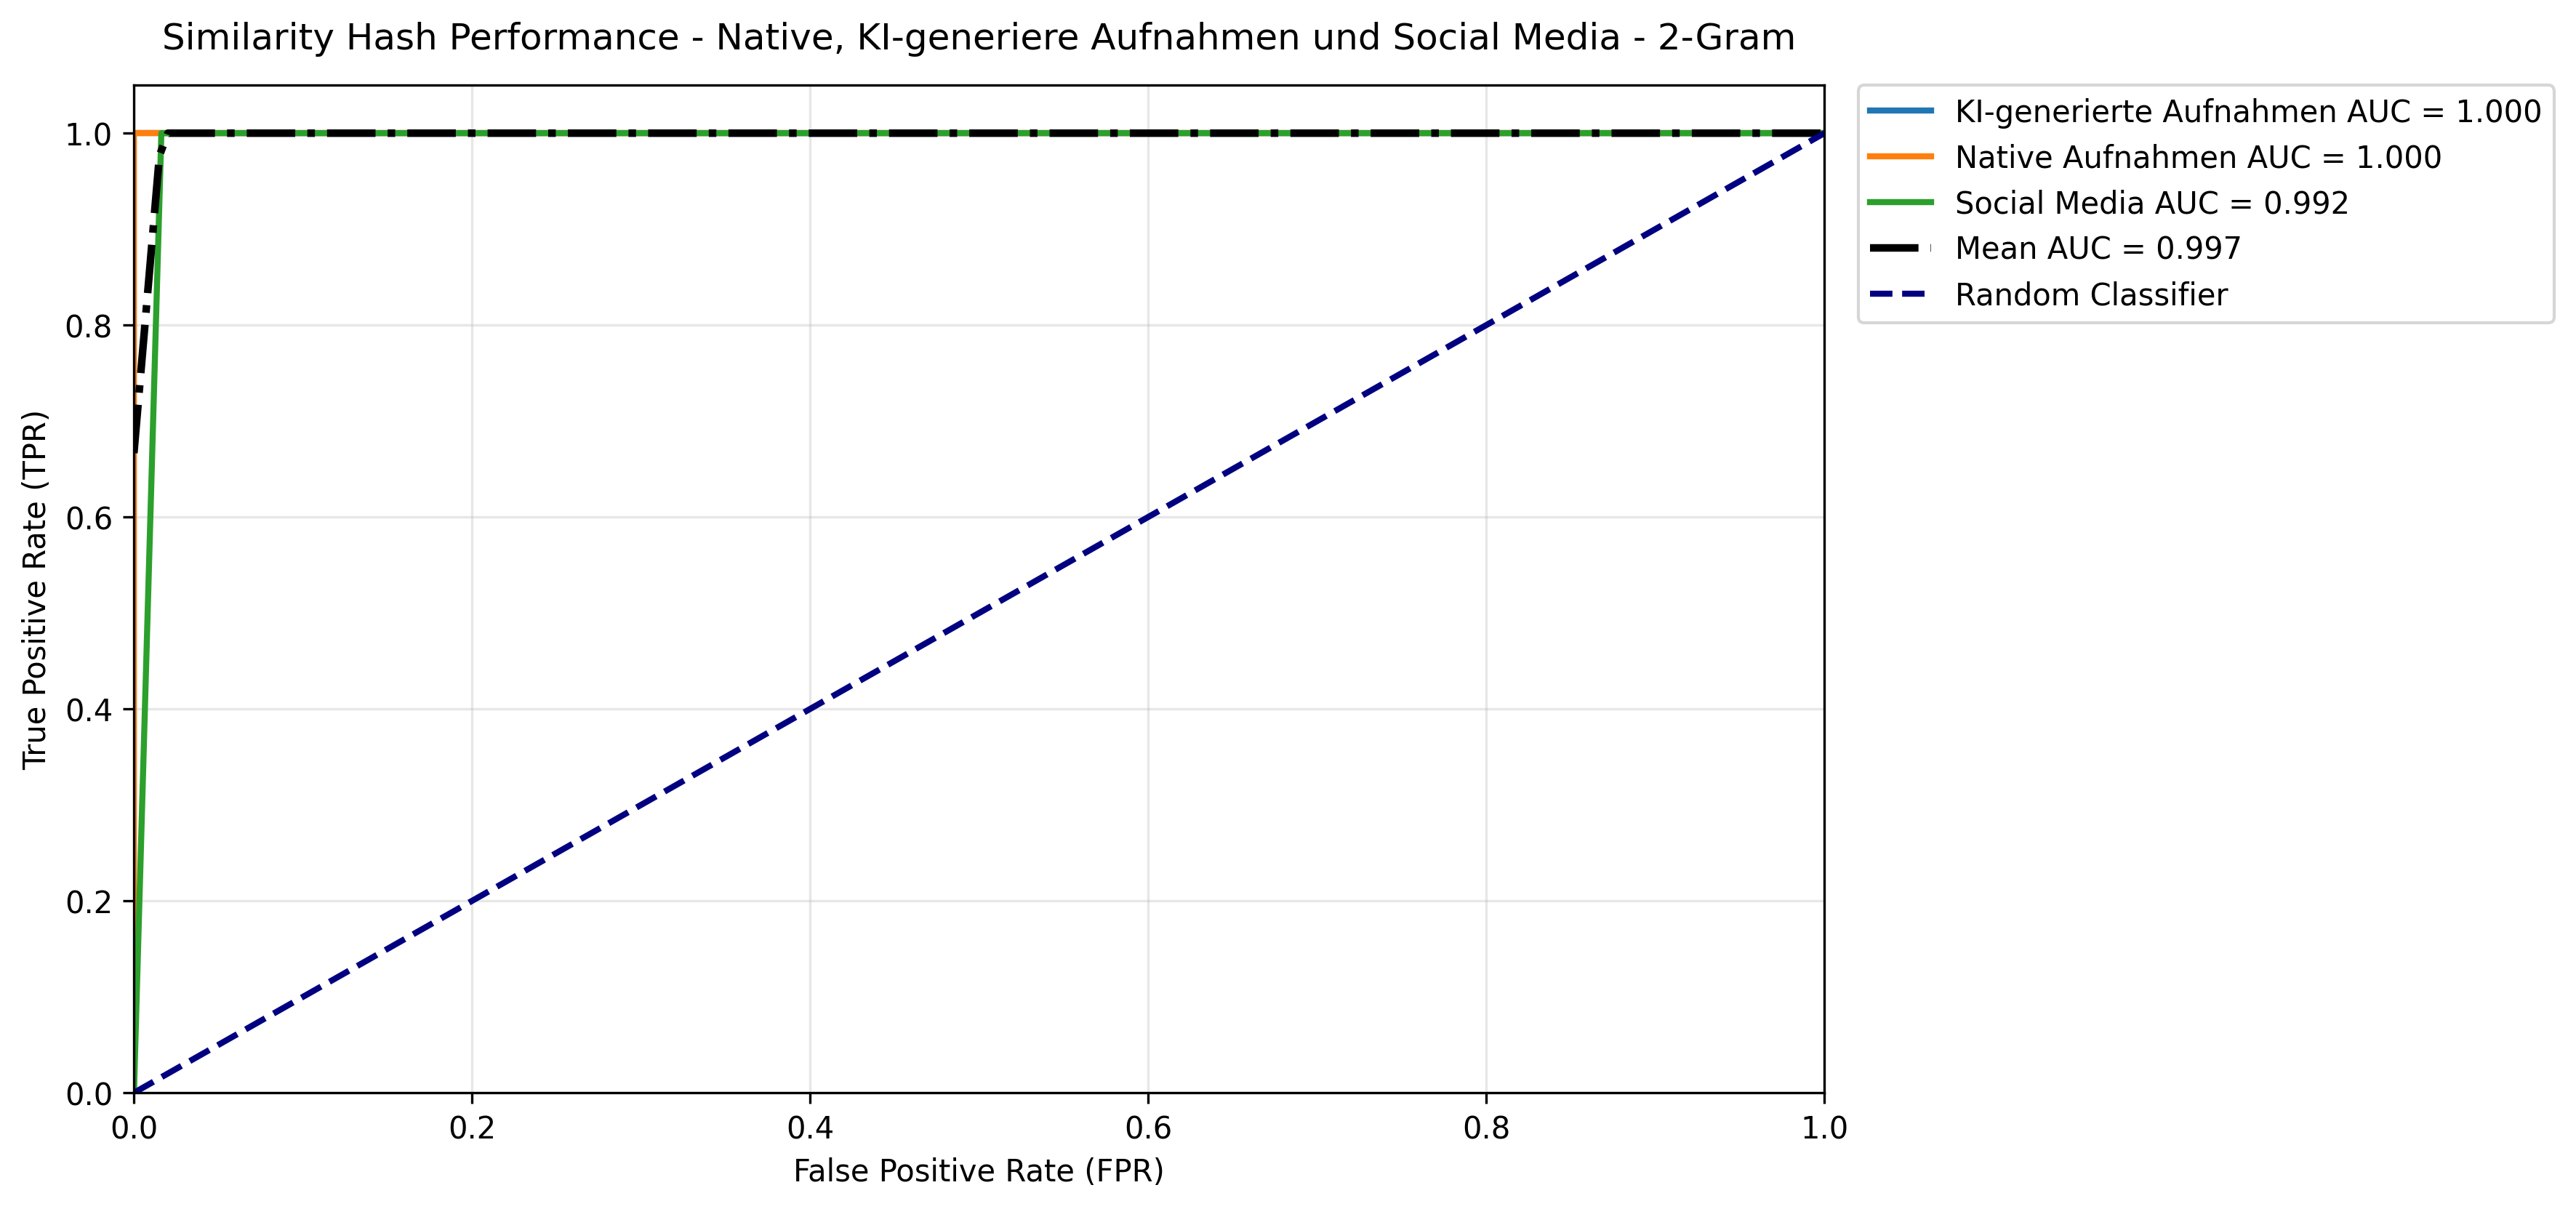
\includegraphics[width=1\linewidth]{grafiken/roc/mixed.png}
    \caption{ROC-Analyse und AUC-Werte zur Identifikation von KI-generierten, nativen und Social Media Videos unter Ausschluss nachträglich bearbeiteter Videos mittels 2-Gramm-Similarity-Hashing (Vision-, EVA-7K- und eigener KI-Datensatz)}
    \label{fig:auc_mixed}
\end{figure}

\begin{figure}[!h]
    \centering
    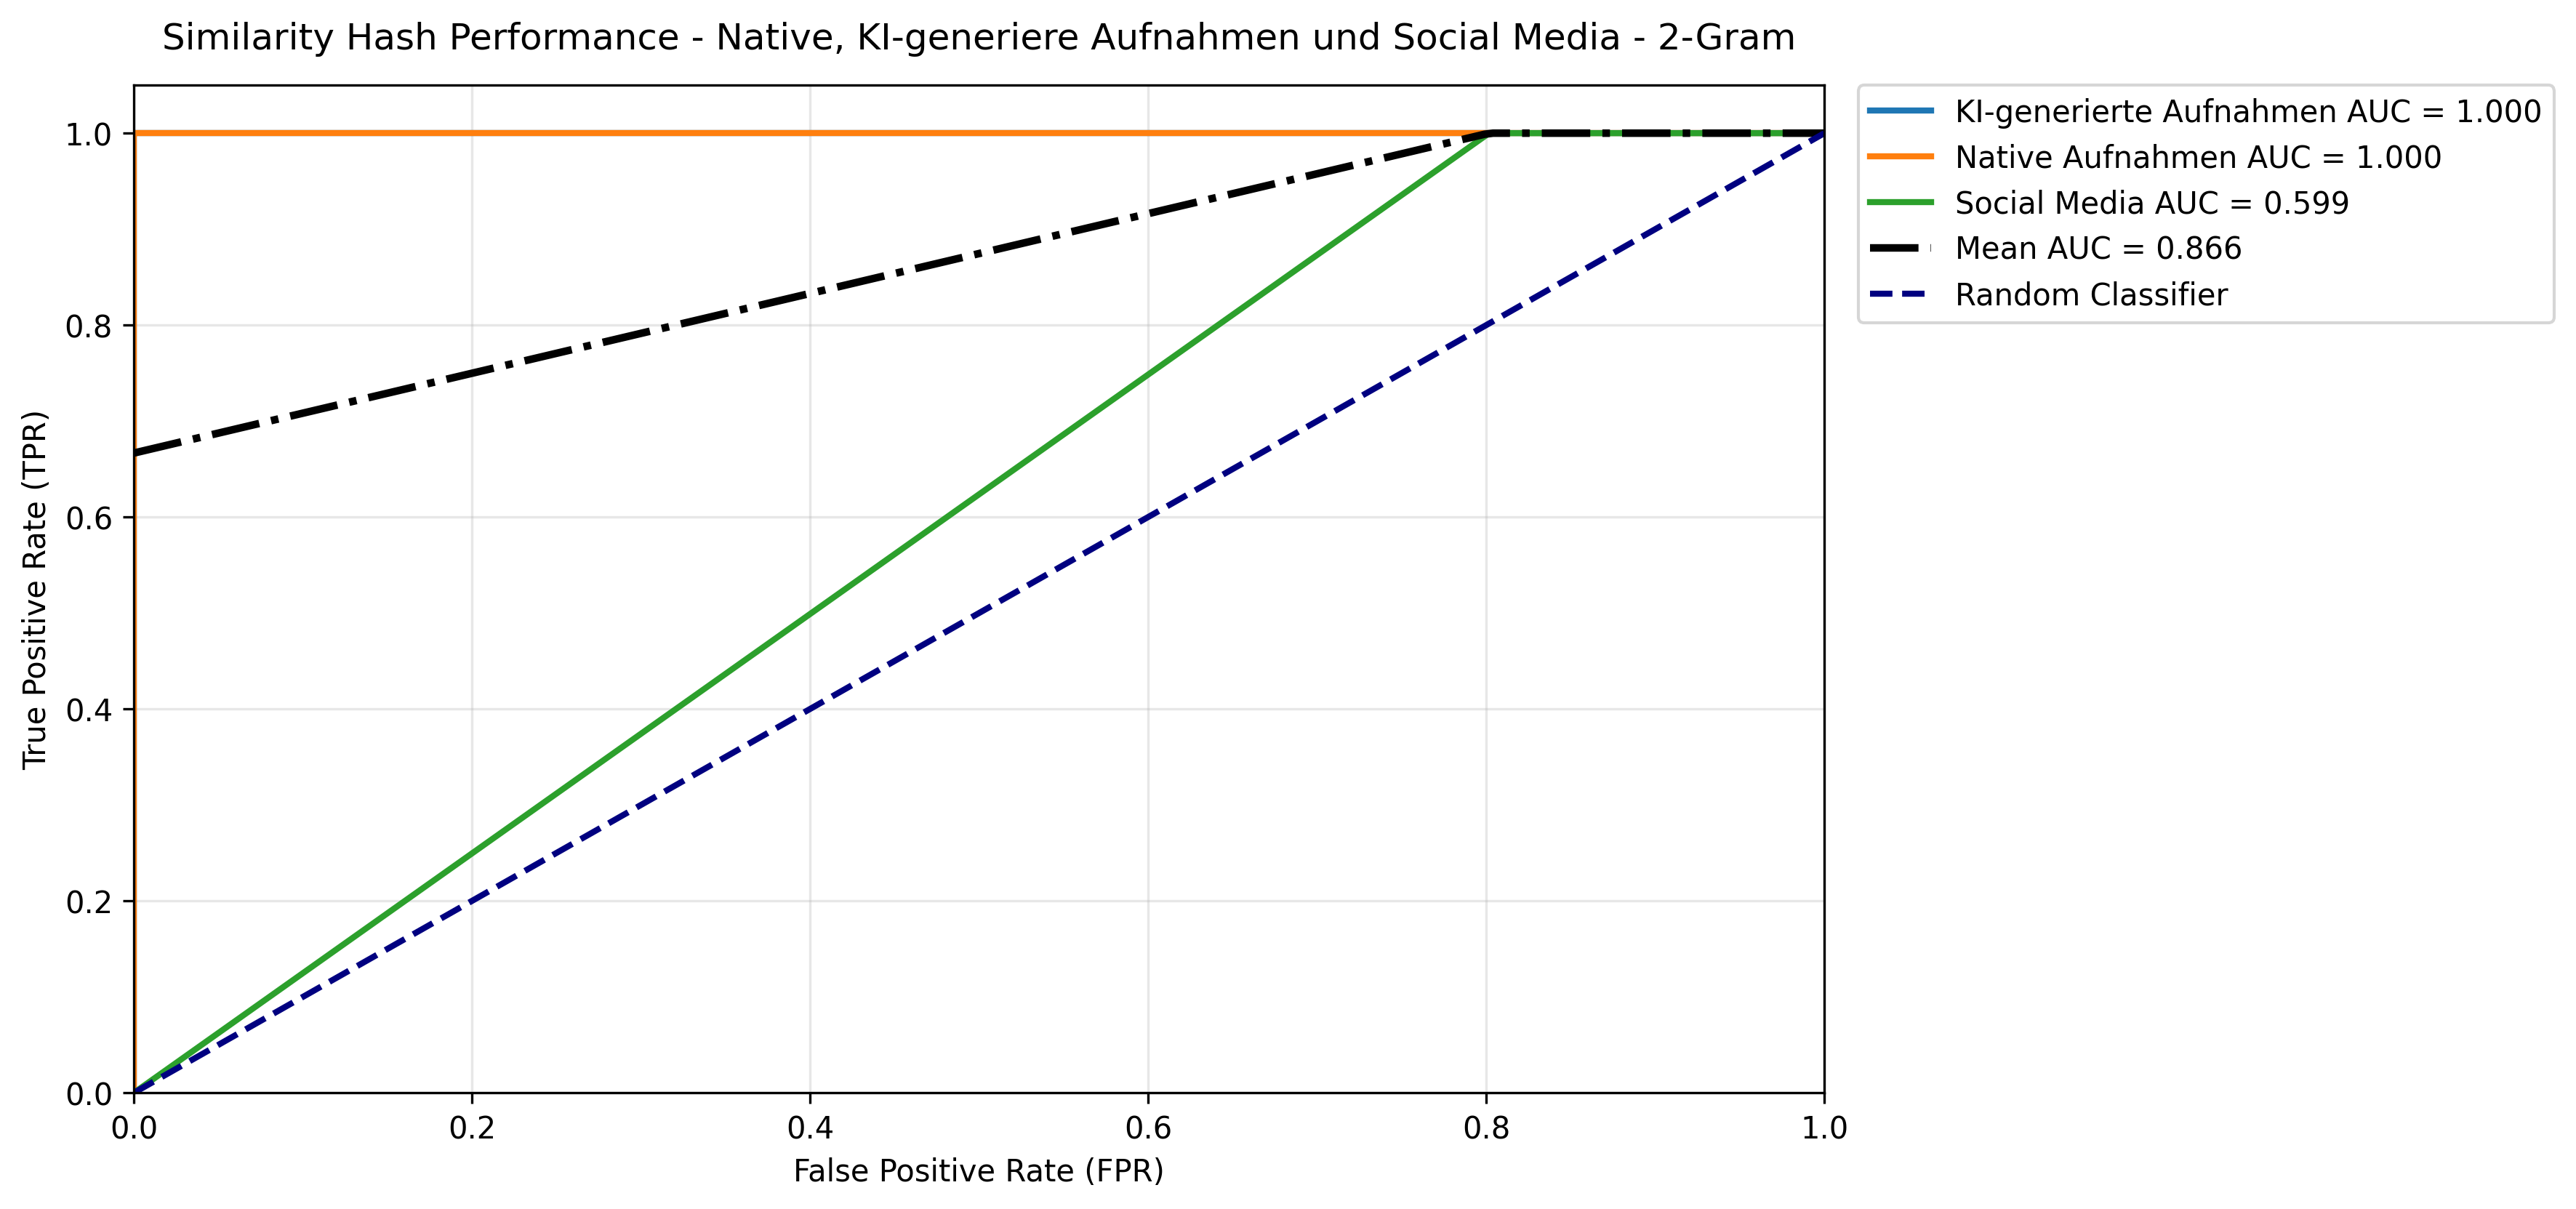
\includegraphics[width=1\linewidth]{grafiken/roc/mixed2.png}
    \caption{ROC-Analyse und AUC-Werte zur Identifikation von KI-generierten, nativen und Social Media Videos mittels 2-Gramm-Similarity-Hashing (Vision-, EVA-7K- und eigener KI-Datensatz)}
    \label{fig:auc_mixed2}
\end{figure}

Die Evaluation zur Identifikation der spezifischen Bearbeitungssoftware (siehe \cref{fig:auc_bearbeitungen}) offenbart jedoch eine signifikante methodische Schwäche des Verfahrens, welche sich in einem AUC-Wert von 0.635 niederschlägt. Bei der Klassifikation manipulierter Videos aus dem EVA-7K-Datensatz, die unter anderem mit Programmen wie Avidemux, ExifTool, FFmpeg, Kdenlive und Adobe Premiere bearbeitet wurden, wird lediglich eine marginale Trennschärfe (AUC-Werte zwischen 0.641 und 0.709) erreicht. Diese Limitierung ist mathematisch direkt auf die Eigenschaften des verwendeten asymmetrischen Tversky-Index zurückzuführen. Da dieser Index explizit so konfiguriert ist, dass er das Fehlen von Container-Boxen in der zu untersuchenden Testdatei nicht bestraft, können softwareseitig bedingte Reduktionen der Metadatenstruktur (Tampering) nicht als distinktes Abweichungsmerkmal erkannt werden \cite[Kap. 3.5]{klier_media_2025}. Folglich wird ein bearbeitetes Video, dem durch den Export lediglich Atome entnommen wurden, fälschlicherweise mit einer nahezu maximalen Ähnlichkeit zur Originalquelle bewertet, was die Erkennungsleistung für Manipulationen massiv herabstuft.\\

TODO: Mixed 2 ergänzen -> \cref{fig:auc_mixed2} (auch in Tabelle oben)

Im deutlichen Kontrast dazu belegt die finale übergeordnete Auswertung (siehe \cref{fig:auc_mixed}) eine hohe Klassifikationsleistung bei der Separation der drei fundamentalen Video-Kategorien. Die Unterscheidung zwischen nativen Aufnahmen, Social-Media-Videos und KI-generierten Inhalten verzeichnet einen AUC-Wert von 0.997. Native Kameraaufnahmen sowie vollständig synthetische Inhalte werden hierbei jeweils fehlerfrei mit einem AUC von 1.000 identifiziert, während die Erkennung von Social-Media-Videos einen Wert von 0.992 erreicht. Dieses Resultat validiert, dass sich Containerstrukturen von Smartphone-Kameras, die serverseitigen Codierungspipelines sozialer Netzwerke sowie die Algorithmen generativer KI-Modelle auf der syntaktischen Ebene der MP4-Container fundamental voneinander unterscheiden und dies eine präzise sowie skalierbare Vorfilterung mittels 2-Gramm-Similarity-Hashing ermöglicht wird.

%%%

\section{Kritische Würdigung und methodische Limitationen}

Hinsichtlich der algorithmischen Effizienz und Skalierbarkeit sind die Ergebnisse des Verfahrens als hochgradig ausreichend und zielführend zu bewerten. Gegenüber qualitativen und baumbasierten Strukturanalysen, die beim Abgleich mit Referenzdaten oftmals eine rechenintensive lineare Komplexität aufweisen, bietet das vorliegende Modell entscheidende architektonische Vorteile. Die Komprimierung der extrahierten Strukturmerkmale in einen kompakten Similarity Digest ermöglicht performante Vergleiche großer Datenmengen und liefert somit einen effizienten Ansatz zur Bewältigung der kontinuierlich wachsenden forensischen Datenflut. Die Ergebnisse für die Vorfilterung (die Erkennung von nativen, Social-Media- und KI-Klassen) sowie für die Marken-Identifikation (SCI) sind exzellent und beweisen die Eignung des Verfahrens für Erstbewertungsverfahren.

Trotz dieser Skalierbarkeit offenbaren sich bei der funktionalen Trennschärfe signifikante methodische Limitationen, wodurch die Ergebnisse für spezifische Untersuchungsziele als unzureichend eingestuft werden müssen. Eine gravierende Schwachstelle manifestiert sich bei der Identifikation von Bearbeitungssoftware (MTI) sowie der generellen Manipulationserkennung, welche lediglich einen AUC-Wert von 0.635 erreicht. Diese Unzulänglichkeit ist direkt auf die mathematischen Eigenschaften des verwendeten asymmetrischen Tversky-Index zurückzuführen. Da dieser Index das Fehlen spezifischer Container-Boxen in der Testdatei nicht bestraft, wird eine softwareseitige Reduktion der Metadatenstruktur durch das Similarity Hashing nicht als distinktes Abweichungsmerkmal klassifiziert. Konkurrierende quantitative Verfahren, welche auf Entscheidungsbäumen basieren und absolute Worthäufigkeiten erfassen, sind hier deutlich überlegen und folglich für die Manipulationserkennung zu präferieren \cite[Kap. 5]{xiang_forensic_2021}.

Eine weitere Einschränkung zeigt sich bei der Klassifikation von KI-Inhalten. Die mangelhafte Trennschärfe zwischen bildbasierten Deepfakes und vollständig synthetisierten Text-to-Video-Inhalten (AUC 0.546) belegt, dass eine rein syntaktische Separation dieser Erzeugungsarten auf Container-Ebene durch das 2-Gramm-Hashing nicht realisierbar ist. Daraus ist abzuleiten, dass KI-Plattformen unabhängig vom initialen Input identische, standardisierte Muxing-Prozesse für die MP4-Generierung anwenden, wodurch keine klassifizierbaren Differenzen in der reinen Container-Grammatik entstehen.

Zusätzlich wird die Präzision auf der Modell-Ebene durch hohe Falsch-Positiv-Raten limitiert, welche durch die Nutzung identischer Betriebssystem-Komponenten hervorgerufen werden. Die strukturelle Ununterscheidbarkeit spezifischer Smartphones (wie bestimmte OnePlus- und Huawei-Modelle) begründet sich in der Verwendung identischer Android-Media-Framework-Implementierungen, welche herstellerübergreifend dieselbe Topologie erzeugen \cite[Kap. 5.4.6]{yang_comprehensive_2025}. Die daraus resultierende strukturelle Angleichung lässt sich durch eine isolierte syntaktische Analyse nicht auflösen.

Zusammenfassend lässt sich die vierte Teilforschungsfrage dahingehend beantworten, dass die Ergebnisse des Similarity Hashing für die Gruppierung von Erzeugerquellen und die schnelle Identifikation unmodifizierter Originale hinreichend belastbar und ausreichend sind. Für feingranulare forensische Fragestellungen, insbesondere den Nachweis von Videomanipulationen durch Software-Encoder oder die Differenzierung synthetischer Sub-Kategorien, erweist sich die Methode in ihrer jetzigen Form jedoch als unzureichend.